\documentclass{beamer}

\mode<presentation>
{
  \usetheme{default}      % or try Darmstadt, Madrid, Warsaw, ...
  \usecolortheme{default} % or try albatross, beaver, crane, ...
  \usefonttheme{default}  % or try serif, structurebold, ...
  \setbeamertemplate{navigation symbols}{}
  \setbeamertemplate{caption}[numbered]
} 

\usepackage[utf8]{inputenc}
\usepackage{epstopdf}
\usepackage{graphicx}
\graphicspath{ {../figures/} }
\usepackage{xcolor}
\usepackage{hyperref}
\usepackage{soul} % for \st{...} aka strikethrough
\usepackage{amsmath} % for math ...
% \usepackage{gensymb} % degree and other symbols ...
\usepackage{tikz} % drawing stuff ..
\usepackage{enumitem}
\usepackage{siunitx} %% SI Units
\usetikzlibrary{tikzmark,shapes}

\tikzset{upper node/.style={fill=red!40},
  lower node/.style={ellipse,fill=red!20},
  ul line/.style={thick,red!20},
  upper/.code={\tikzset{upper node/.append style={#1}}},
  lower/.code={\tikzset{lower node/.append style={#1}}},
  line/.code={\tikzset{ul line/.append style={#1}}},
}

%% highlight with explanation beneath, see 
%% https://tex.stackexchange.com/questions/458694/highlighting-part-of-equation-with-text-underneath
\newcounter{HighLight}
\newcommand{\highlightwu}[3][]{%
  \stepcounter{HighLight}
  \tikzset{#1}
  \underset{\underset{\displaystyle\makebox[0pt]{\text{\tikzmarknode[lower node]{below-\theHighLight}{%
    #3}}}}{\phantom{!}}}{\tikzmarknode[upper node]{above-\theHighLight}{#2}}
    \tikz[overlay,remember picture]{\draw[ul line] (above-\theHighLight) --
      (below-\theHighLight);}
}
%% highlight term
\newcommand{\highlight}[2][]{%
  \stepcounter{HighLight}
  \tikzset{#1}
  {\tikzmarknode[upper node]{above-\theHighLight}{\textbf #2}}
}

%% define a box ...
\setbeamercolor{postit}{fg=black,bg=example text.fg!75!black!10!bg}

%% some itemize styles
\newcommand{\citem}{\item[\checkmark]}
\newcommand{\bitem}{\item[\textbullet]}
\newcommand{\ditem}{\item[\textendash]}
\newcommand{\aitem}{\item[\textasteriskcentered]}

\usepackage{natbib}
\bibliographystyle{plainnat}

\title[]{PhD Status}
\author{Xanthos}
\institute{DSO \& IGN}
\date{\today}

\begin{document}

\begin{frame}
  \titlepage
\end{frame}

% Uncomment these lines for an automatically generated outline.
%\begin{frame}{Outline}
%  \tableofcontents
%\end{frame}

\begin{frame}\frametitle{So far ...}\framesubtitle{}
  \begin{itemize}
    \citem Meeting on 15 Oct 2021
  \end{itemize}
\end{frame}

\begin{frame}\frametitle{RINEX observations}\framesubtitle{Observables}
  DORIS RINEX files contain (as observables):
  \begin{itemize}
    \bitem L1 \& L2 phase data
    \bitem C1 \& C2 pseudo range data (only for time-tagging)
    \bitem W1 \& W2 power level data (data screening ?)
    \bitem Relative frequency data
    \bitem P, T \& H meteorological data (later to be used for tropospheric dealy)
  \end{itemize}
  \vspace{.2cm}

  All observations include a complicated set of flags\\
  \vspace{.2cm}
\end{frame}

\begin{frame}\frametitle{RINEX observations}\framesubtitle{Data Screening (1/2)}
  \underline{Observation screening:}\\
  At this point use the observation flags read off from the \(L_{2GHz}\) observation. 
  In case a discontinuity is recorded in the RINEX file, start a new arc and diregard 
  the marked observation.

  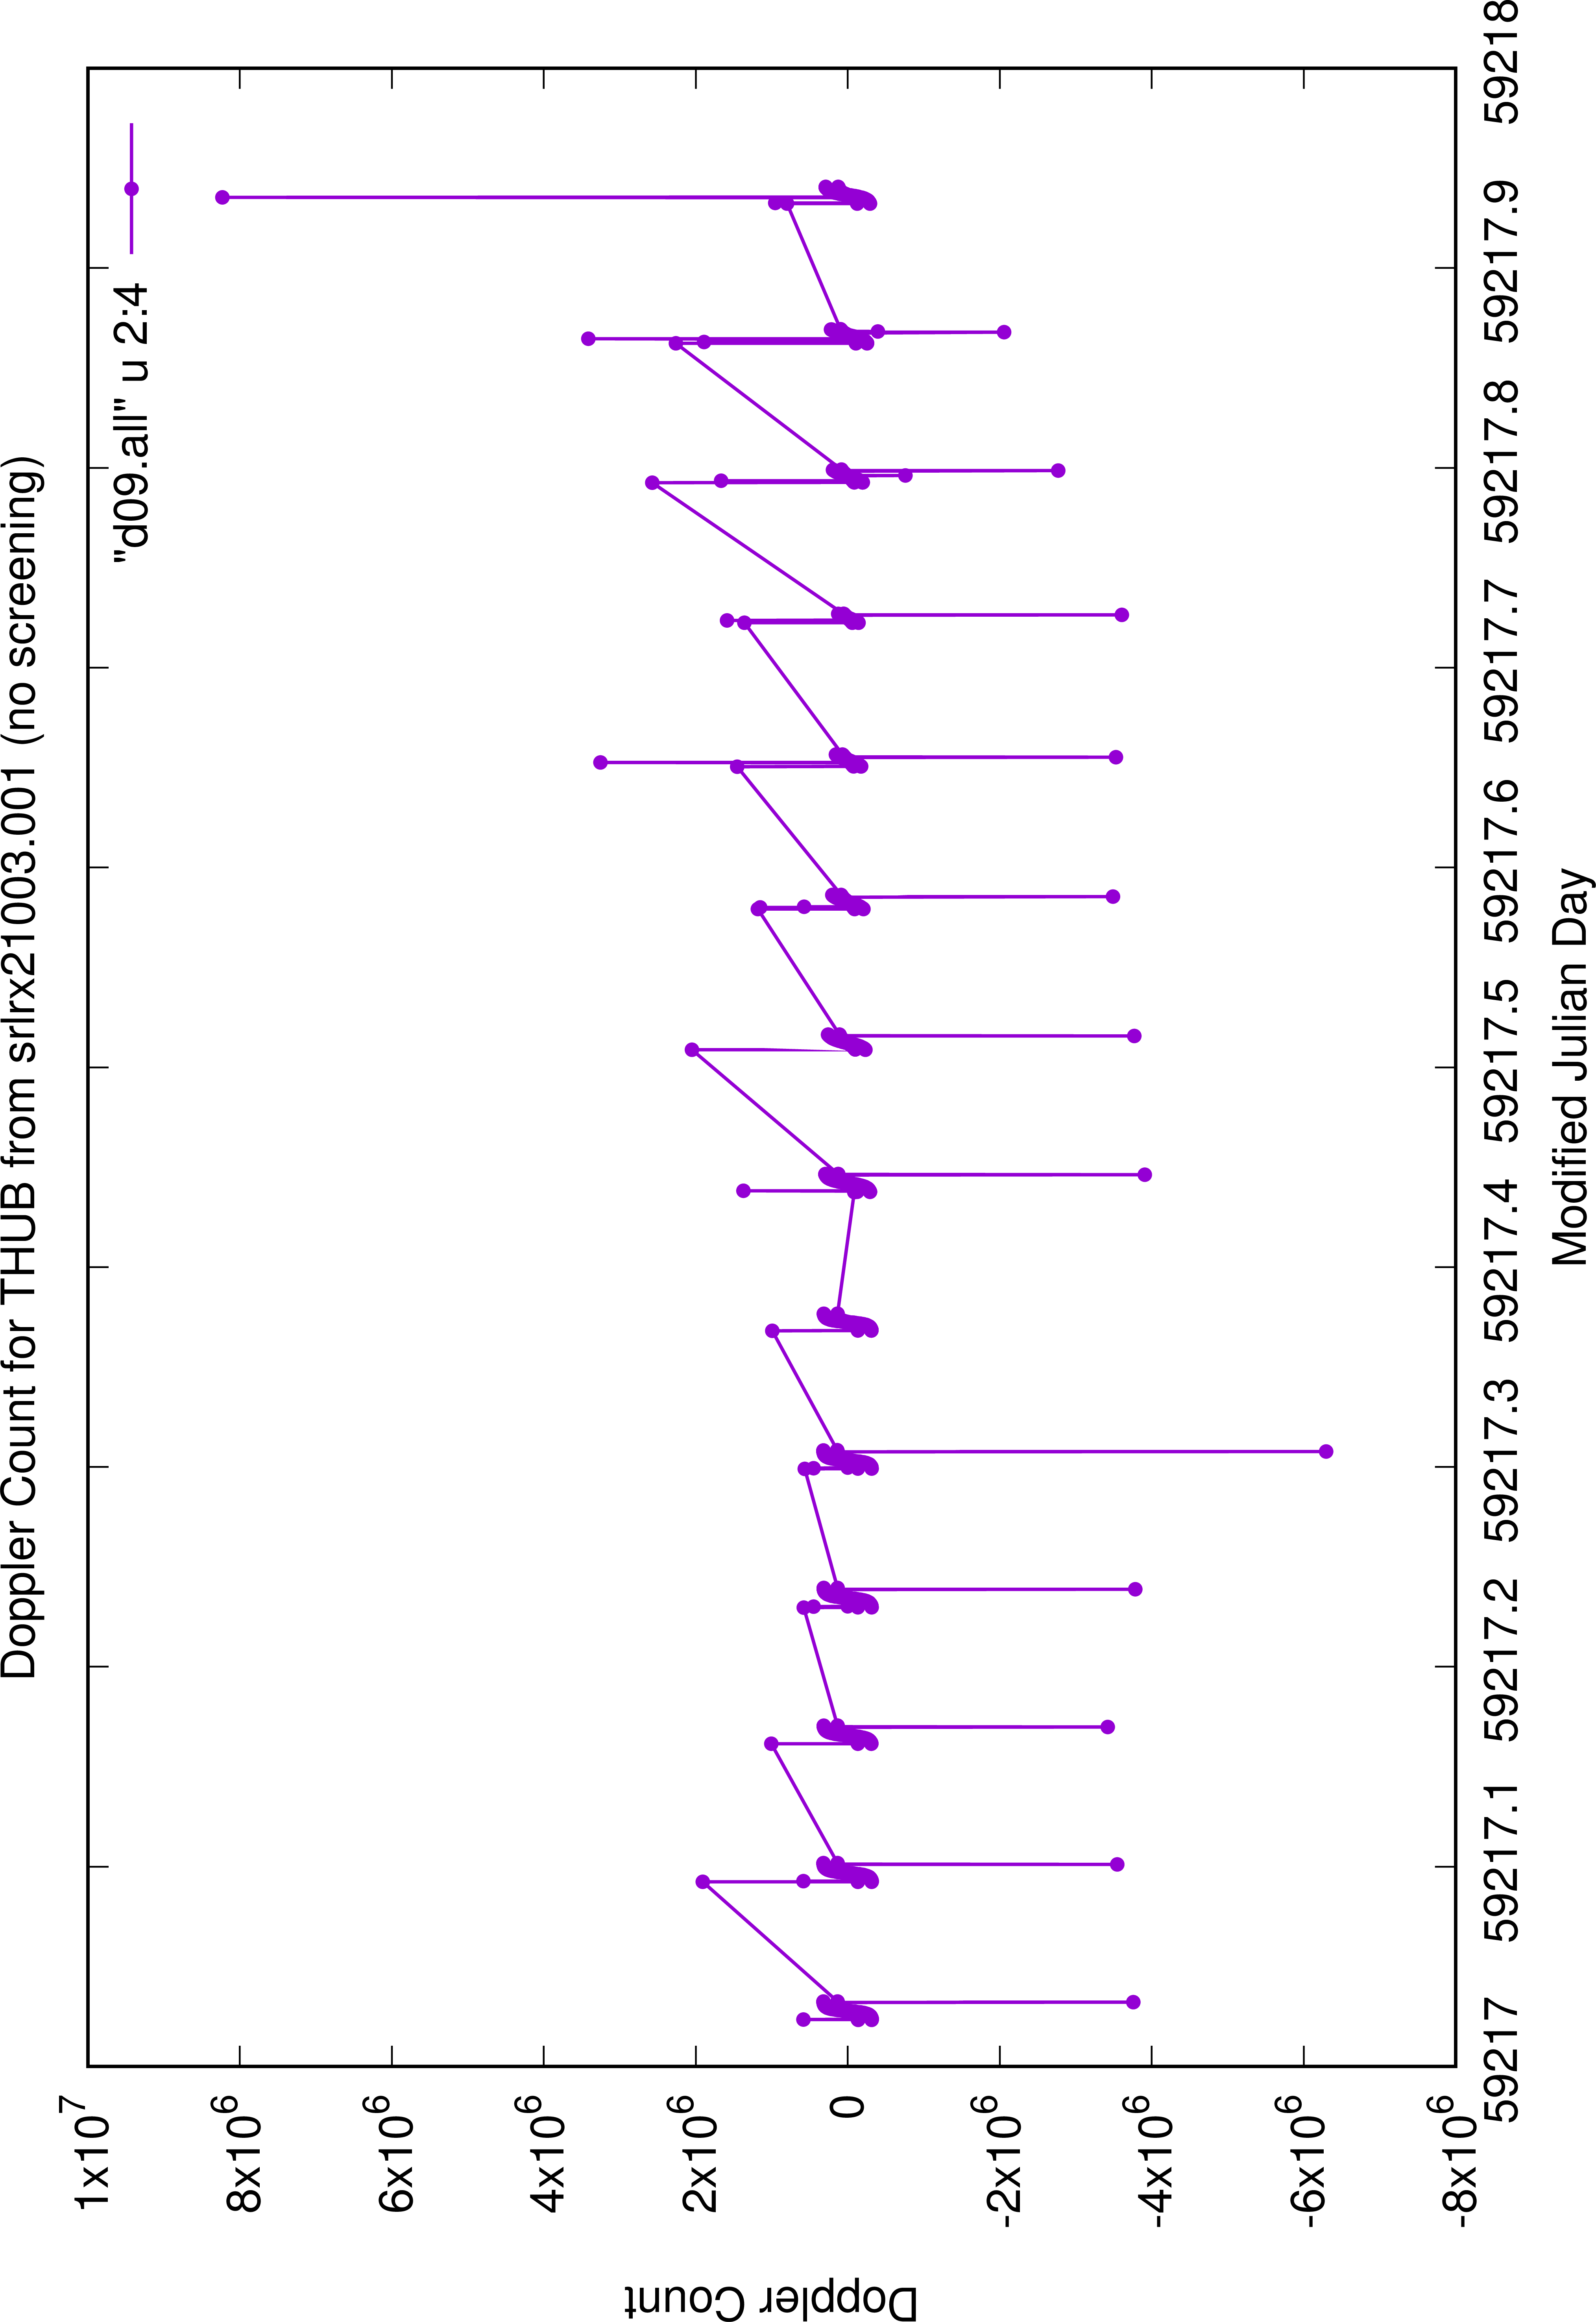
\includegraphics[angle=-90, width=0.50\textwidth]{THUB-srlrx21003.001-allobs}%
  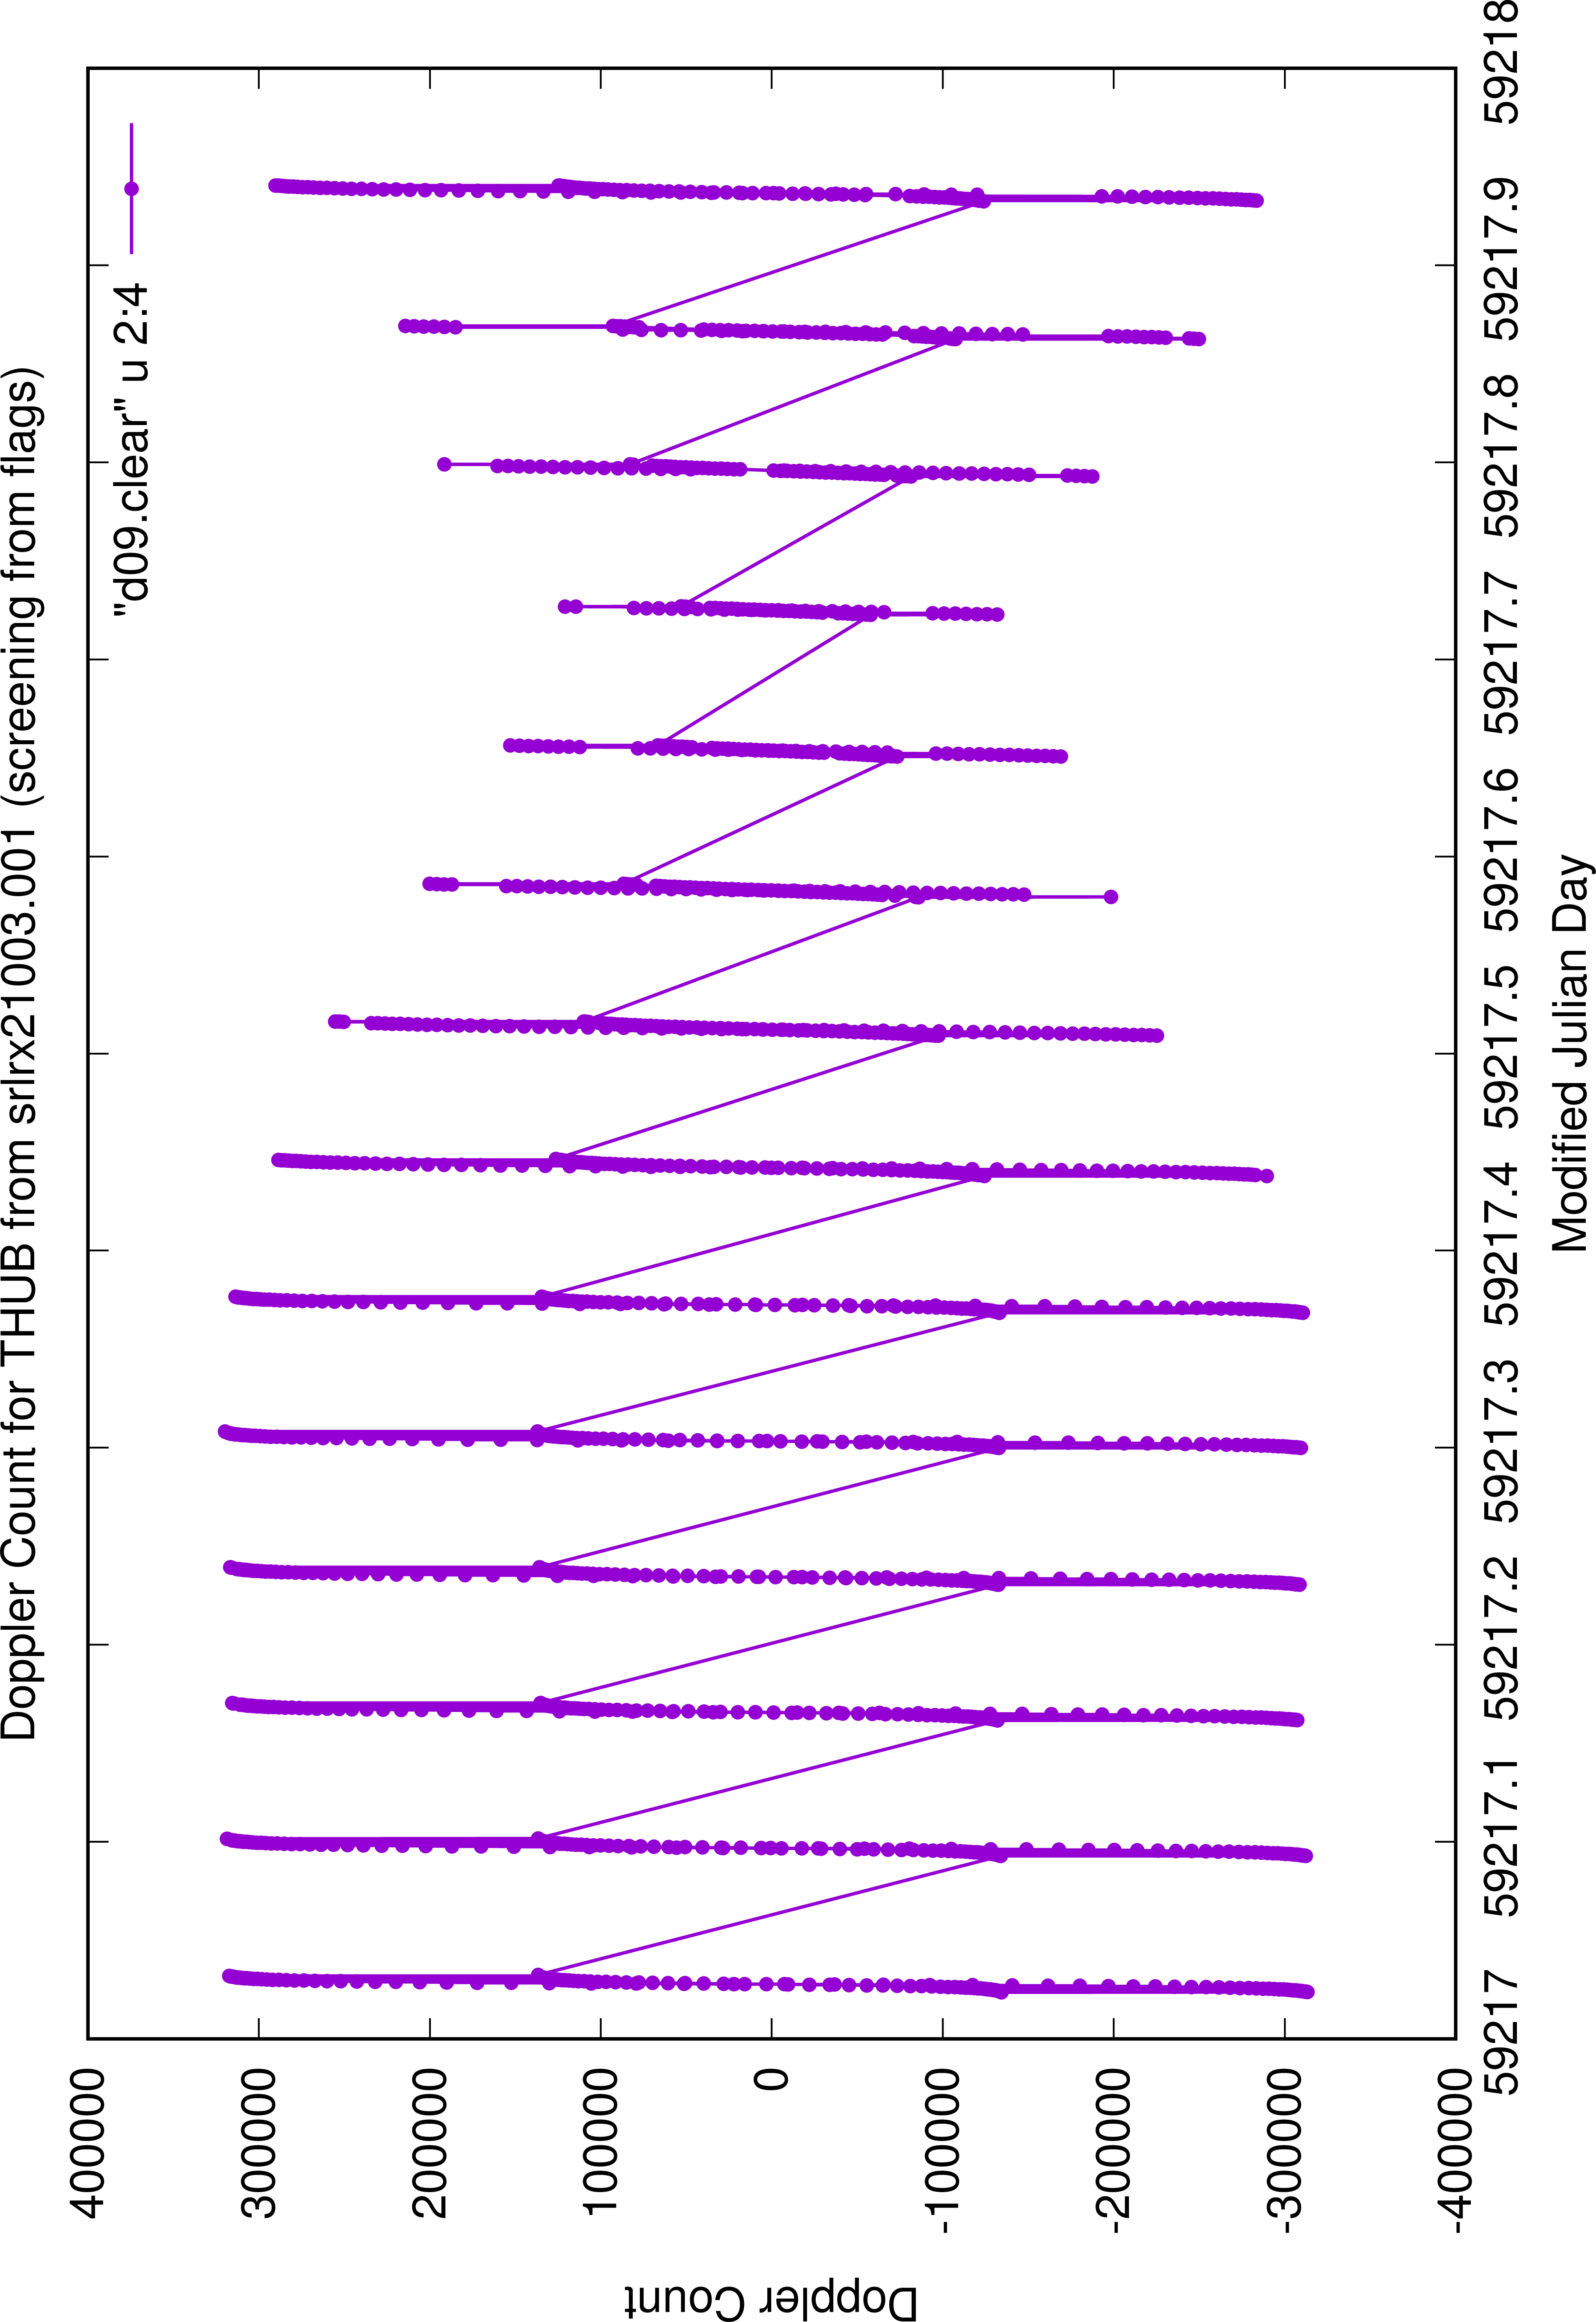
\includegraphics[angle=-90, width=0.50\textwidth]{THUB-srlrx21003.001-screened}

\end{frame}

\begin{frame}\frametitle{RINEX observations}\framesubtitle{Data Screening (2/2)}
\begin{table}
\caption{Flagged $L_{2GHZ}$ observations per RINEX file; some examples}
\label{tab:table}
{\tiny
\begin{tabular}{|c|c|c|c|}
\hline \hline
  RINEX & Satellite & Total $L_{2GHz}$ obs & Flagged $L_{2GHz}$ Obs (\%) \\
  \hline
  srlrx21001.001 & Saral & 34153 & 10.1 \\
  srlrx21002.001 && 34213 & 10.1 \\
  srlrx21003.001 && 3281 & 9.6 \\
  s6arx21001.001 & Sentinel-6A & 3655 & 6.9 \\
  s6arx21002.001 && 3854 & 7.2 \\
  s6arx21003.001 && 3748 & 6.9 \\
  s6arx21004.001 && 3796 & 7.1 \\
  s6arx21005.001 && 3724 & 6.9 \\
  ja3rx21001.001 & Jason-3 & 53115 & 6.9 \\
  ja3rx21002.001 && 53830  & 7.2 \\
  ja3rx21003.001 && 54399 & 6.8 \\
  ja3rx21004.001 && 53243 & 7.2 \\
  ja3rx21005.001 && 54335 & 6.9 \\
\hline\hline
\end{tabular}
}

\begin{itemize}
  \aitem \textcolor{red}{Could later use a more sophisticated algorithm; e.g. linear/polynomial fitting 
  of phase observables (like GNSS, turboedit/MAUPRP)}
\end{itemize}
\end{table}


\end{frame}

\begin{frame}\frametitle{Observation Equation}\framesubtitle{Starting Point}
  The following equation \cite{lemoine-2016} will be the basis for data processing:
  \begin{equation*}
    \label{eq:lem17}
    \left.\begin{aligned}
        u_{measured} & = \frac{c}{f_{e_N}} 
          (f_{e_N} - f_{r_T}
            - \frac{N_{DOP}}{\Delta\tau_r}) 
          + \Delta u_{{REL}_C} 
          + \Delta u_{IONO}\\
        u_{theo} &= \frac{\rho_2 - \rho_1}{\Delta\tau_r} 
          + \Delta u_{TROPO} 
          - \frac{c(\frac{N_{DOP}}{\Delta\tau_r} 
          + f_{r_T})}{f_{e_N}} 
            \frac{\Delta f_e}{f_{e_N}}
    \end{aligned}
\right\}
\end{equation*}

Need to figure out each term in the equation to formulate the observation equation.
\end{frame}

\begin{frame}[shrink=20]\frametitle{Parameters}\framesubtitle{Nominal Frequencies \(f_{r_N}\) and \(f_{e_N}\)}
  \begin{equation*}
    \left.\begin{aligned}
        u_{measured} & = \frac{\textcolor{red}c}{\highlight[upper=ellipse]{f_{e_N}}} 
          (\highlight[upper=ellipse]{f_{e_N}} - f_{r_T}
            - \frac{N_{DOP}}{\Delta\tau_r}) 
          + \Delta u_{{REL}_C} 
          + \Delta u_{IONO}\\
        u_{theo} &= \frac{\rho_2 - \rho_1}{\Delta\tau_r} 
          + \Delta u_{TROPO} 
          - \frac{\textcolor{red}c(\frac{N_{DOP}}{\Delta\tau_r} 
          + f_{r_T})}{\highlight[upper=ellipse]{f_{e_N}}} 
            \frac{\Delta f_e}{f_{e_N}}
    \end{aligned}
\right\}
\end{equation*}

\(f_{e_N}\) is the ``nominal'' (proper) frequency of the emitter. For each 
emitter/beacon, the nominal frequency is: 
\begin{equation*}
  f_N = A \cdot F_0 (\frac{3}{4} + \frac{87 \cdot k}{5 \cdot 2^{26}})
\end{equation*}
where:
\begin{align*}
A = \left\{%
    \begin{array}{cc}
      543e0 & for \hspace{2mm} f = S_1 = 2GHz \\
      107e0 & for \hspace{2mm} f = U_2 = 400 MHz
    \end{array}%
  \right.
  \end{align*}

  \(F_0 = USO \hspace{2mm} frequency = 5 \cdot 10^6 Hz\)

and \(k\) is the station frequency shift factor (\textit{signed integer, usually 0}); 
\textbf{this last value is extracted from the RINEX file(s)}.
\end{frame}

\begin{frame}\frametitle{Parameters}\framesubtitle{Doppler Count \(N_{DOP}\)}
  \begin{equation*}
    \left.\begin{aligned}
        u_{measured} & = \frac{\textcolor{red}c}{\textcolor{red}{f_{e_N}}} 
          (\textcolor{red}{f_{e_N}} - f_{r_T}
            - \frac{\highlight[upper=ellipse]{N_{DOP}}}{\Delta\tau_r}) 
          + \Delta u_{{REL}_C} 
          + \Delta u_{IONO}\\
        u_{theo} &= \frac{\rho_2 - \rho_1}{\Delta\tau_r} 
          + \Delta u_{TROPO} 
          - \frac{\textcolor{red}c(\frac{\highlight[upper=ellipse]{N_{DOP}}}{\Delta\tau_r} 
          + f_{r_T})}{\textcolor{red}{f_{e_N}}} 
            \frac{\Delta f_e}{f_{e_N}}
    \end{aligned}
\right\}
\end{equation*}%

\(N_{DOP}\) is the Doppler count, aka the difference of two consecutive phase observations 
on the 2 GHz carrier (for the same beacon). 
\textbf{We can form this value using the RINEX file(s)}. Normally, ``consecutive'' observations 
are 3 or 7 sec away.

\begin{beamercolorbox}[wd=\textwidth,rounded=true,shadow=true]{postit}
In the RINEX files, this Doppler count is the difference between two phase measurements
done at different time tags in the proper time-scale of the receiver.
\end{beamercolorbox}

\end{frame}

\begin{frame}\frametitle{Parameters}\framesubtitle{Proper Receiver Frequency \(f_{r_T}\) (1/2)}
  \begin{equation*}
    \left.\begin{aligned}
        u_{measured} & = \frac{\color{red}c}{\color{red}f_{e_N}} 
          (\textcolor{red}{f_{e_N}} - 
            \highlight[upper=ellipse]{f_{r_T}} -
            \frac{\color{red}N_{DOP}}{\Delta\tau_r}) + 
          \Delta u_{{REL}_C} + 
          \Delta u_{IONO}\\
        u_{theo} &= \frac{\rho_2 - \rho_1}{\Delta\tau_r} + 
          \Delta u_{TROPO} - 
          \frac{\textcolor{red}c(\frac{\textcolor{red}{N_{DOP}}}{\Delta\tau_r} + 
          \highlight[upper=ellipse]{f_{r_T}})}{\textcolor{red}{f_{e_N}}} 
          \highlightwu[upper={ellipse, fill=blue!30}, line={black,latex-}]{\frac{\Delta f_e}{f_{e_N}}}{estimate}
    \end{aligned}
\right\}
\end{equation*}

\begin{itemize}
  \bitem nominal frequencies (\(f_{{[r|e]}_{N}}\)) are not equal to the ``true'' frequencies (\(f_{{[r|e]}_{T}}\))
  \bitem in the observation equation we need to have the ``true'' frequencies, \(f_{e_T} = f_{e_N} (1 + \Delta f_e / f_{e_N})\)
  \bitem \(\Delta f_e\) and \(\Delta f_r\) are 100\% correlated, only one of them can be ajusted; choose \(\Delta f_e\)
  \bitem we need good a-priori estimates of \(\Delta f_r\)
\end{itemize}
\end{frame}

\begin{frame}\frametitle{Parameters}\framesubtitle{Proper Receiver Frequency \(f_{r_T}\) (2/2)}
  We need a value for  \(\Delta f_r / f_{r_N}\) (every epoch). The values can be 
  estimated or \textbf{extracted from RINEX files}, under the ``F'' measurement (one value 
  per obervation block). It is recommended to smooth values over one or more days.

  \begin{center}
    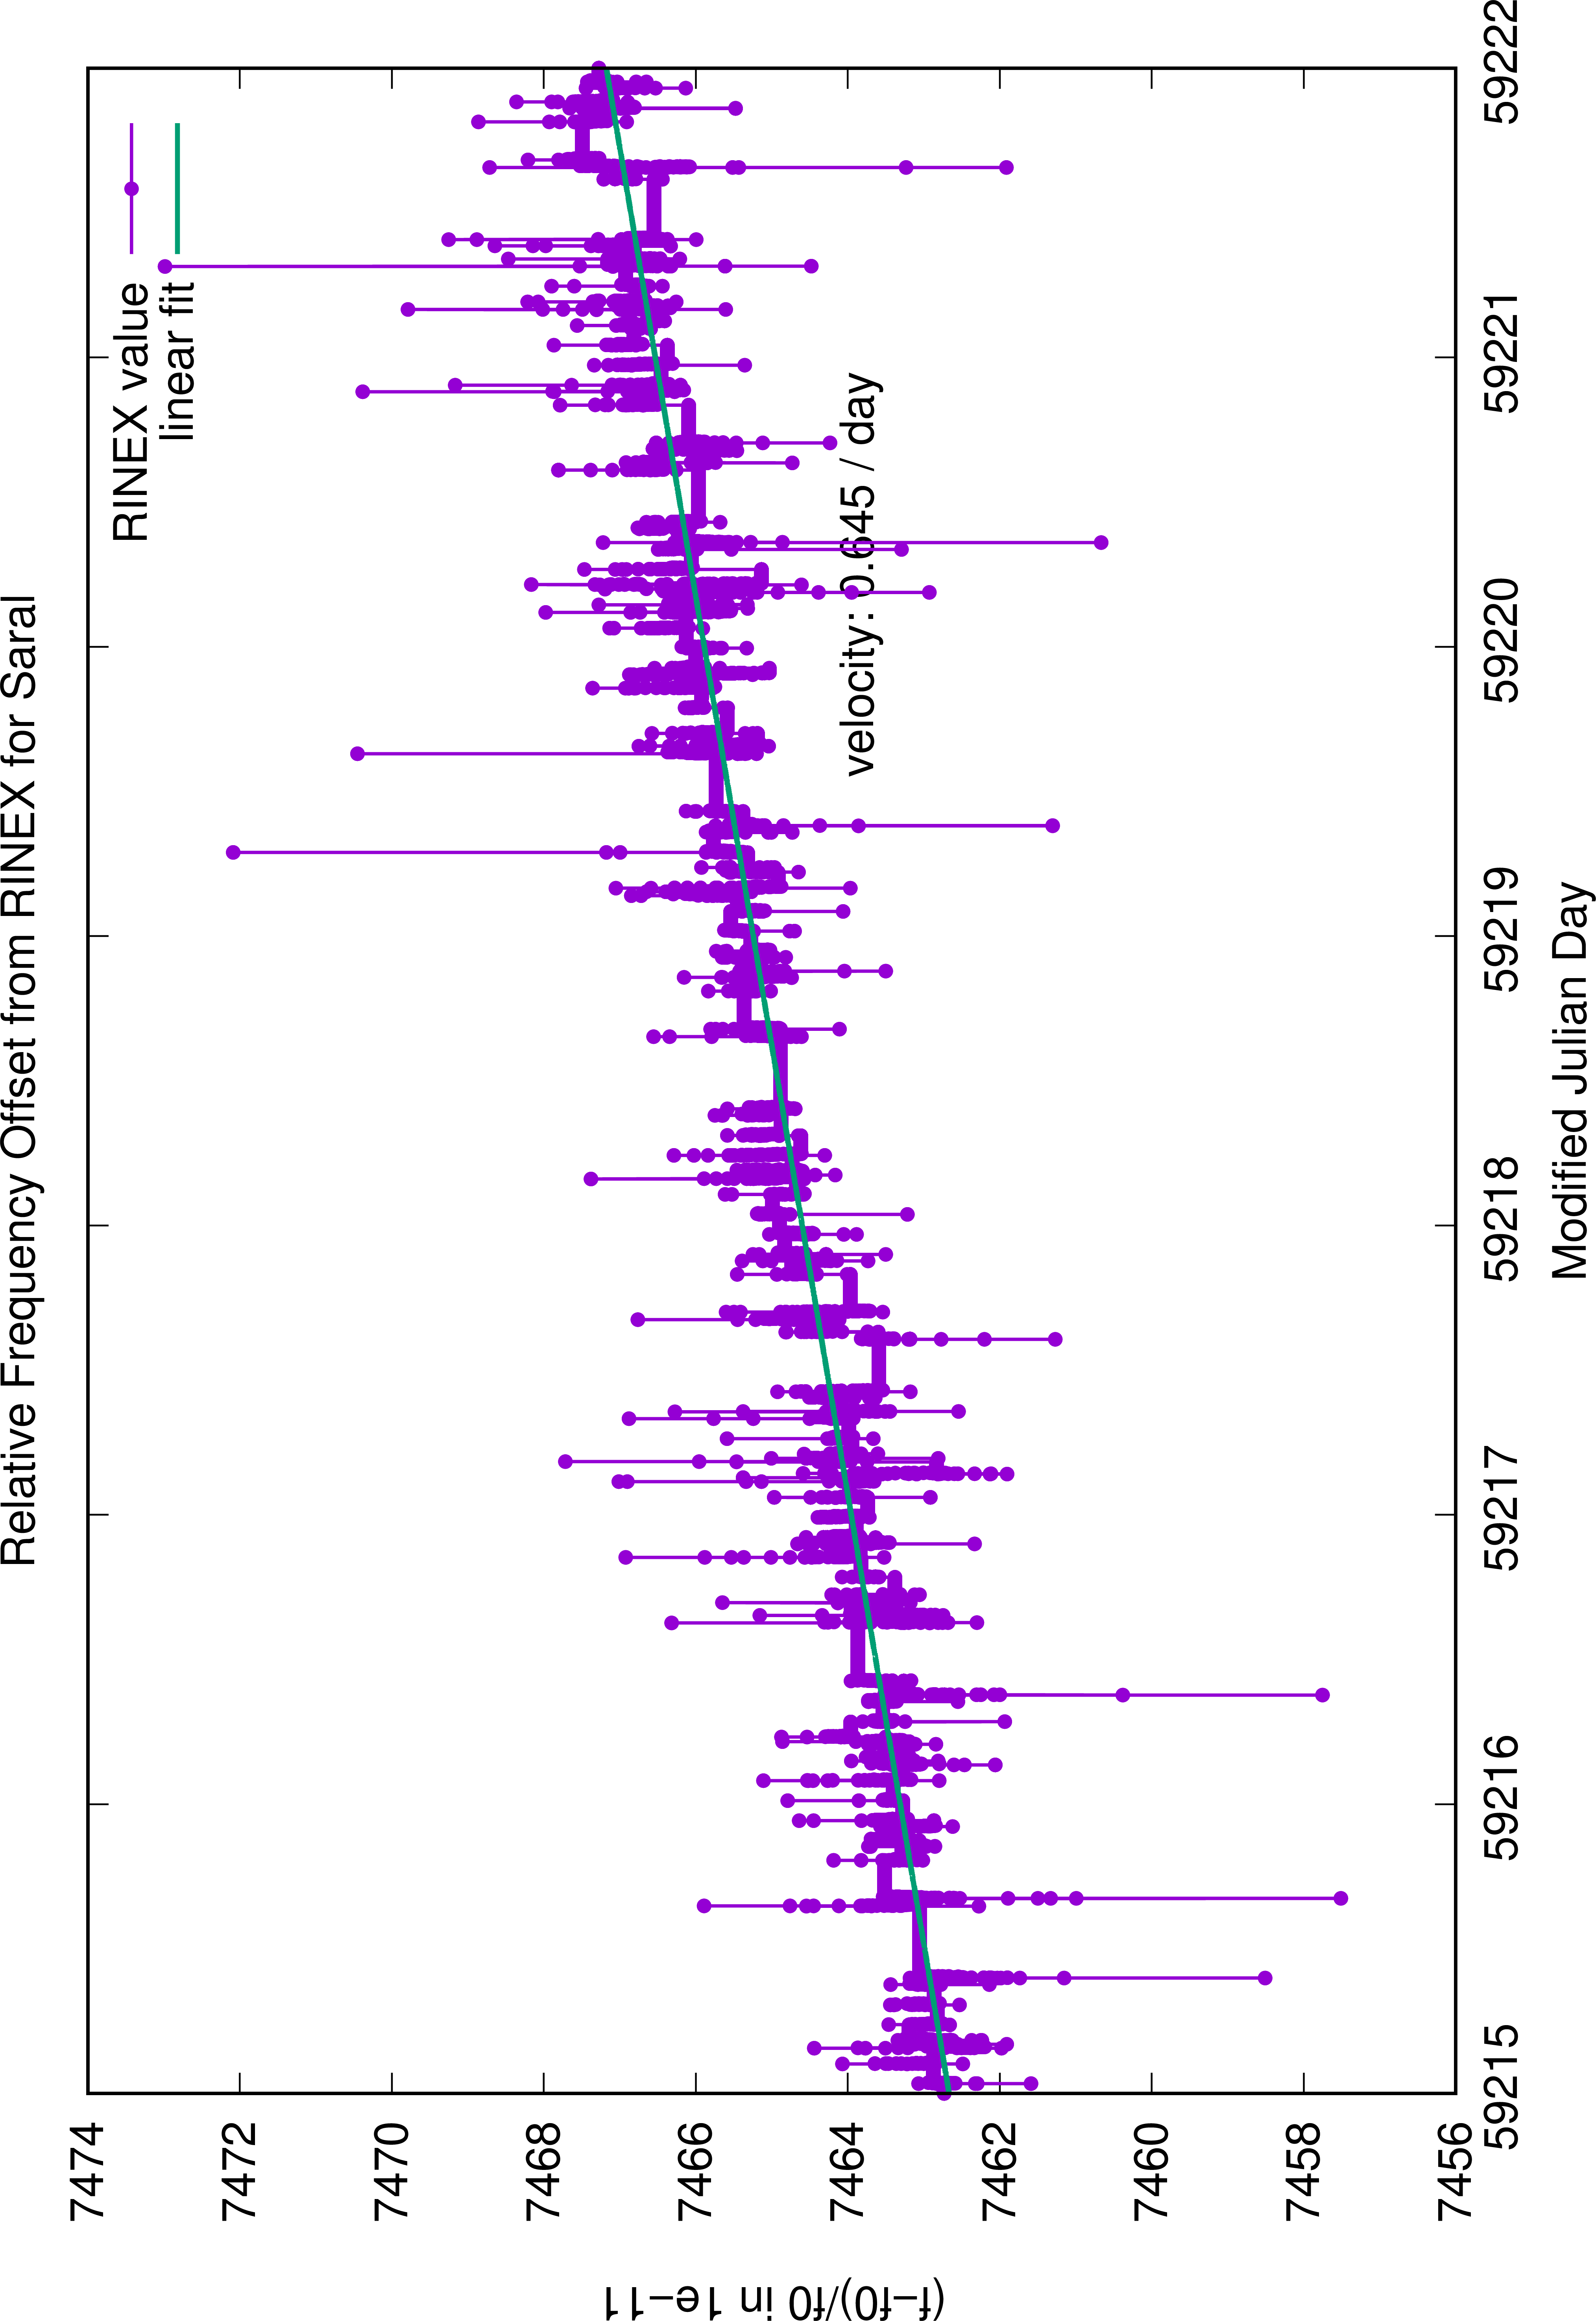
\includegraphics[scale=.3, angle=-90]{Saral-RinexRfo}
  \end{center}
\end{frame}

\begin{frame}\frametitle{Parameters}\framesubtitle{Delta Time \(\Delta\tau_r\)}
  \begin{equation*}
    \left.\begin{aligned}
        u_{measured} & = \frac{\color{red}c}{\color{red}f_{e_N}} 
          (\textcolor{red}{f_{e_N}} - 
            \textcolor{red}{f_{r_T}} -
            \frac{\color{red}N_{DOP}}{
        \tikz[baseline]{
          \node[fill=red!35, ellipse, anchor=base]
          {$\Delta\tau_r$};
        }} +
          \Delta u_{{REL}_C} + 
          \Delta u_{IONO}\\
        u_{theo} &= \frac{\rho_2 - \rho_1}{
          } + 
          \Delta u_{TROPO} - 
          \frac{\textcolor{red}c(\frac{\textcolor{red}{N_{DOP}}}{
        \tikz[baseline]{
          \node[fill=red!35, ellipse, anchor=base]
          {$\Delta\tau_r$};
          }} +
          \textcolor{red}{f_{r_T}})}{\textcolor{red}{f_{e_N}}} 
          \textcolor{blue}{\frac{\Delta f_e}{f_{e_N}}}
    \end{aligned}
\right\}
\end{equation*}

\(\Delta\tau_r = \tau_{r2} - \tau_{r1}\), where \(\tau_{r1}\) is the beginning of reception 
of the the 1\textsubscript{st} cycle by the receiver, and 
\(\tau_{r2}\) the end of reception of the N\textsubscript{th} cycle by the receiver, \underline{in the 
proper time scale of the receiver}.

\end{frame}

\begin{frame}\frametitle{Parameters}\framesubtitle{Satellite-Beacon distance \(\rho\) (1/3)}
  \begin{equation*}
    \left.\begin{aligned}
        u_{measured} & = \frac{\color{red}c}{\color{red}f_{e_N}} 
          (\textcolor{red}{f_{e_N}} - 
            \textcolor{red}{f_{r_T}} -
            \frac{\color{red}N_{DOP}}{\textcolor{red}{\Delta\tau_r}}) + 
          \Delta u_{{REL}_C} + 
          \Delta u_{IONO}\\
        u_{theo} &= \frac{\tikz[baseline]{
          \node[fill=red!35, ellipse, anchor=base]
          {$\rho_2 - \rho_1$};
        }
        }{\textcolor{red}{\Delta\tau_r}} + 
          \Delta u_{TROPO} - 
          \frac{\textcolor{red}c(\frac{\textcolor{red}{N_{DOP}}}{
            \textcolor{red}{\Delta\tau_r}
          } + 
          \textcolor{red}{f_{r_T}})}{\textcolor{red}{f_{e_N}}} 
          \textcolor{blue}{\frac{\Delta f_e}{f_{e_N}}}
    \end{aligned}
\right\}
\end{equation*}

where:
  \begin{equation*}
    \rho_i = \Vert \vec{X}_{sat}|_{t \gets\tau_{ri}} - \vec{X}_{beacon} \Vert , i=1,2
  \end{equation*}
We need beacon and satellite position vectors for each epoch (aka every \(\tau_{r1}\) 
and \(\tau_{r2}\)). Both in the same, earth-fixed, reference frame ...

\end{frame}

\begin{frame}\frametitle{Parameters}\framesubtitle{Satellite-Beacon distance \(\rho\) (2/3)}
  \textbf{Satellite position vector for \(\tau_{r1}\) and \(\tau_{r2}\),  \(\vec{X}_{sat}|_{t \gets\tau_{ri}}\)}:\\
  \vspace{.2cm}
  Interpolate from IDS-pubished Sp3 files. Usually, these files contain more than one days; 
  they record the satellite's state vector (both position and velocity) typically every 
  60 sec, in ITRF.\\
  \vspace{.2cm}
  Interpolation is performed via (slightly modified) Neville's method. Typically 9 
  neighbourhing points are used (6 on each side).

\end{frame}

\begin{frame}\frametitle{Parameters}\framesubtitle{Satellite-Beacon distance \(\rho\) (3/3)}
  \textbf{Beacon position vector for \(\tau_{r1}\) and \(\tau_{r2}\),  \(\vec{X}_{beacon}\)}:\\
  \vspace{.2cm}
  \underline{Simplification:} for now we assume no significant displacement of the beacon 
  within one day. This is generally not true (see tides, etc ...); later model using iers2010 
  models.\\
  \vspace{.2cm}
  Beacon coordinates are extrapolated using the IDS-published DPOD SINEX file.\\
  \vspace{.1cm}
  \begin{beamercolorbox}[wd=\textwidth,rounded=true,shadow=true]{postit}
  PDOP is a “DORIS extension of the ITRF for Precise Orbit Determination”
  estimated and delivered by the IDS Combination Center.
  \end{beamercolorbox}

\end{frame}

\begin{frame}\frametitle{Parameters}\framesubtitle{Tropospheric Delay \(\Delta u_{TROPO}\) (1/)}
  \begin{equation*}
    \left.\begin{aligned}
        u_{measured} & = \frac{\color{red}c}{\color{red}f_{e_N}} 
          (\textcolor{red}{f_{e_N}} - 
            \textcolor{red}{f_{r_T}} -
            \frac{\color{red}N_{DOP}}{\textcolor{red}{\Delta\tau_r}}) + 
          \Delta u_{{REL}_C} + 
          \Delta u_{IONO}\\
        u_{theo} &= \frac{\textcolor{red}{\rho_2 - \rho_1}}{\textcolor{red}{\Delta\tau_r}} + 
        \tikz[baseline]{
          \node[fill=red!35, ellipse, anchor=base]
          {$\Delta u_{TROPO}$};
        }
          - \frac{\textcolor{red}c(\frac{\textcolor{red}{N_{DOP}}}{
            \textcolor{red}{\Delta\tau_r}
          } + 
          \textcolor{red}{f_{r_T}})}{\textcolor{red}{f_{e_N}}} 
          \textcolor{blue}{\frac{\Delta f_e}{f_{e_N}}}
    \end{aligned}
\right\}
\end{equation*}

We choose to model the tropospheric delay using the (empirical) GPT3 mapping functions, 
that is:
\begin{equation*}
  \Delta u_{TROPO} = \Delta {L_{h}}^{z} \cdot mf_h(\epsilon) + \Delta {L_{w}}^{z} \cdot mf_w(\epsilon)
\end{equation*}

\end{frame}

\begin{frame}\frametitle{Parameters}\framesubtitle{Tropospheric Delay \(\Delta u_{TROPO}\) (2/)}
Derivation follows \cite{Landskron2018}

For each beacon
\begin{enumerate}[label=\textbf{T.\arabic*},ref=T.\arabic*]
  \item \label{gpt3call} call \texttt{gpt3(mjd, $\phi$, $\lambda$)}; this returns a 
  list of parameters including the \textbf{mapping coefficients \texttt{$\alpha _h$, $\alpha _w$}}
  
  \item call \texttt{vmf3(\(\alpha _h, \alpha _w\), ...)} to get \textbf{\(mf_h(\epsilon)\) and \(mf_w(\epsilon)\)}
  
  \item use \begin{equation*}
    \Delta {L_{h}}^{z} = \frac{0.0022768 \cdot p}{1-0.00266 \cdot \cos(2\phi) - 0.28 \cdot 10^{-6} \cdot h_{ell}}
  \end{equation*}
  where $p$ is the pressure at the site, which can be obtained from either \ref{gpt3call} 
  or the RINEX file (each epoch) and $h_{ell}$ is the ellipsoidal height.
  
  \item use \begin{equation*}
    \Delta {L_{w}}^{z} = 10^{-6} \cdot ( k_2 + \frac{k_3}{T_m}) \cdot \frac{R_d e}{g_m (\lambda +1)}
  \end{equation*}
  where $e$ is water vapour pressure, $T_m$ is mean 
  temperature weighted with the water vapor and $\lambda$ is the water vapour 
  decrease factor; all of these are obtained from the call to \ref{gpt3call}
\end{enumerate}

\end{frame}

\begin{frame}\frametitle{Parameters}\framesubtitle{Tropospheric Delay \(\Delta u_{TROPO}\) (3/)}
  We need the pressure (at each beacon) to compute  \(\Delta {L_{h}}^{z}\); we can either 
  use the values provided in the RINEX files, or the one computed from GPT3.
  One day of Saral data; Pressure (hPa) and \(ZTD_H\) (m) from RINEX Vs GPT3 derived values ...
  %\begin{center}
    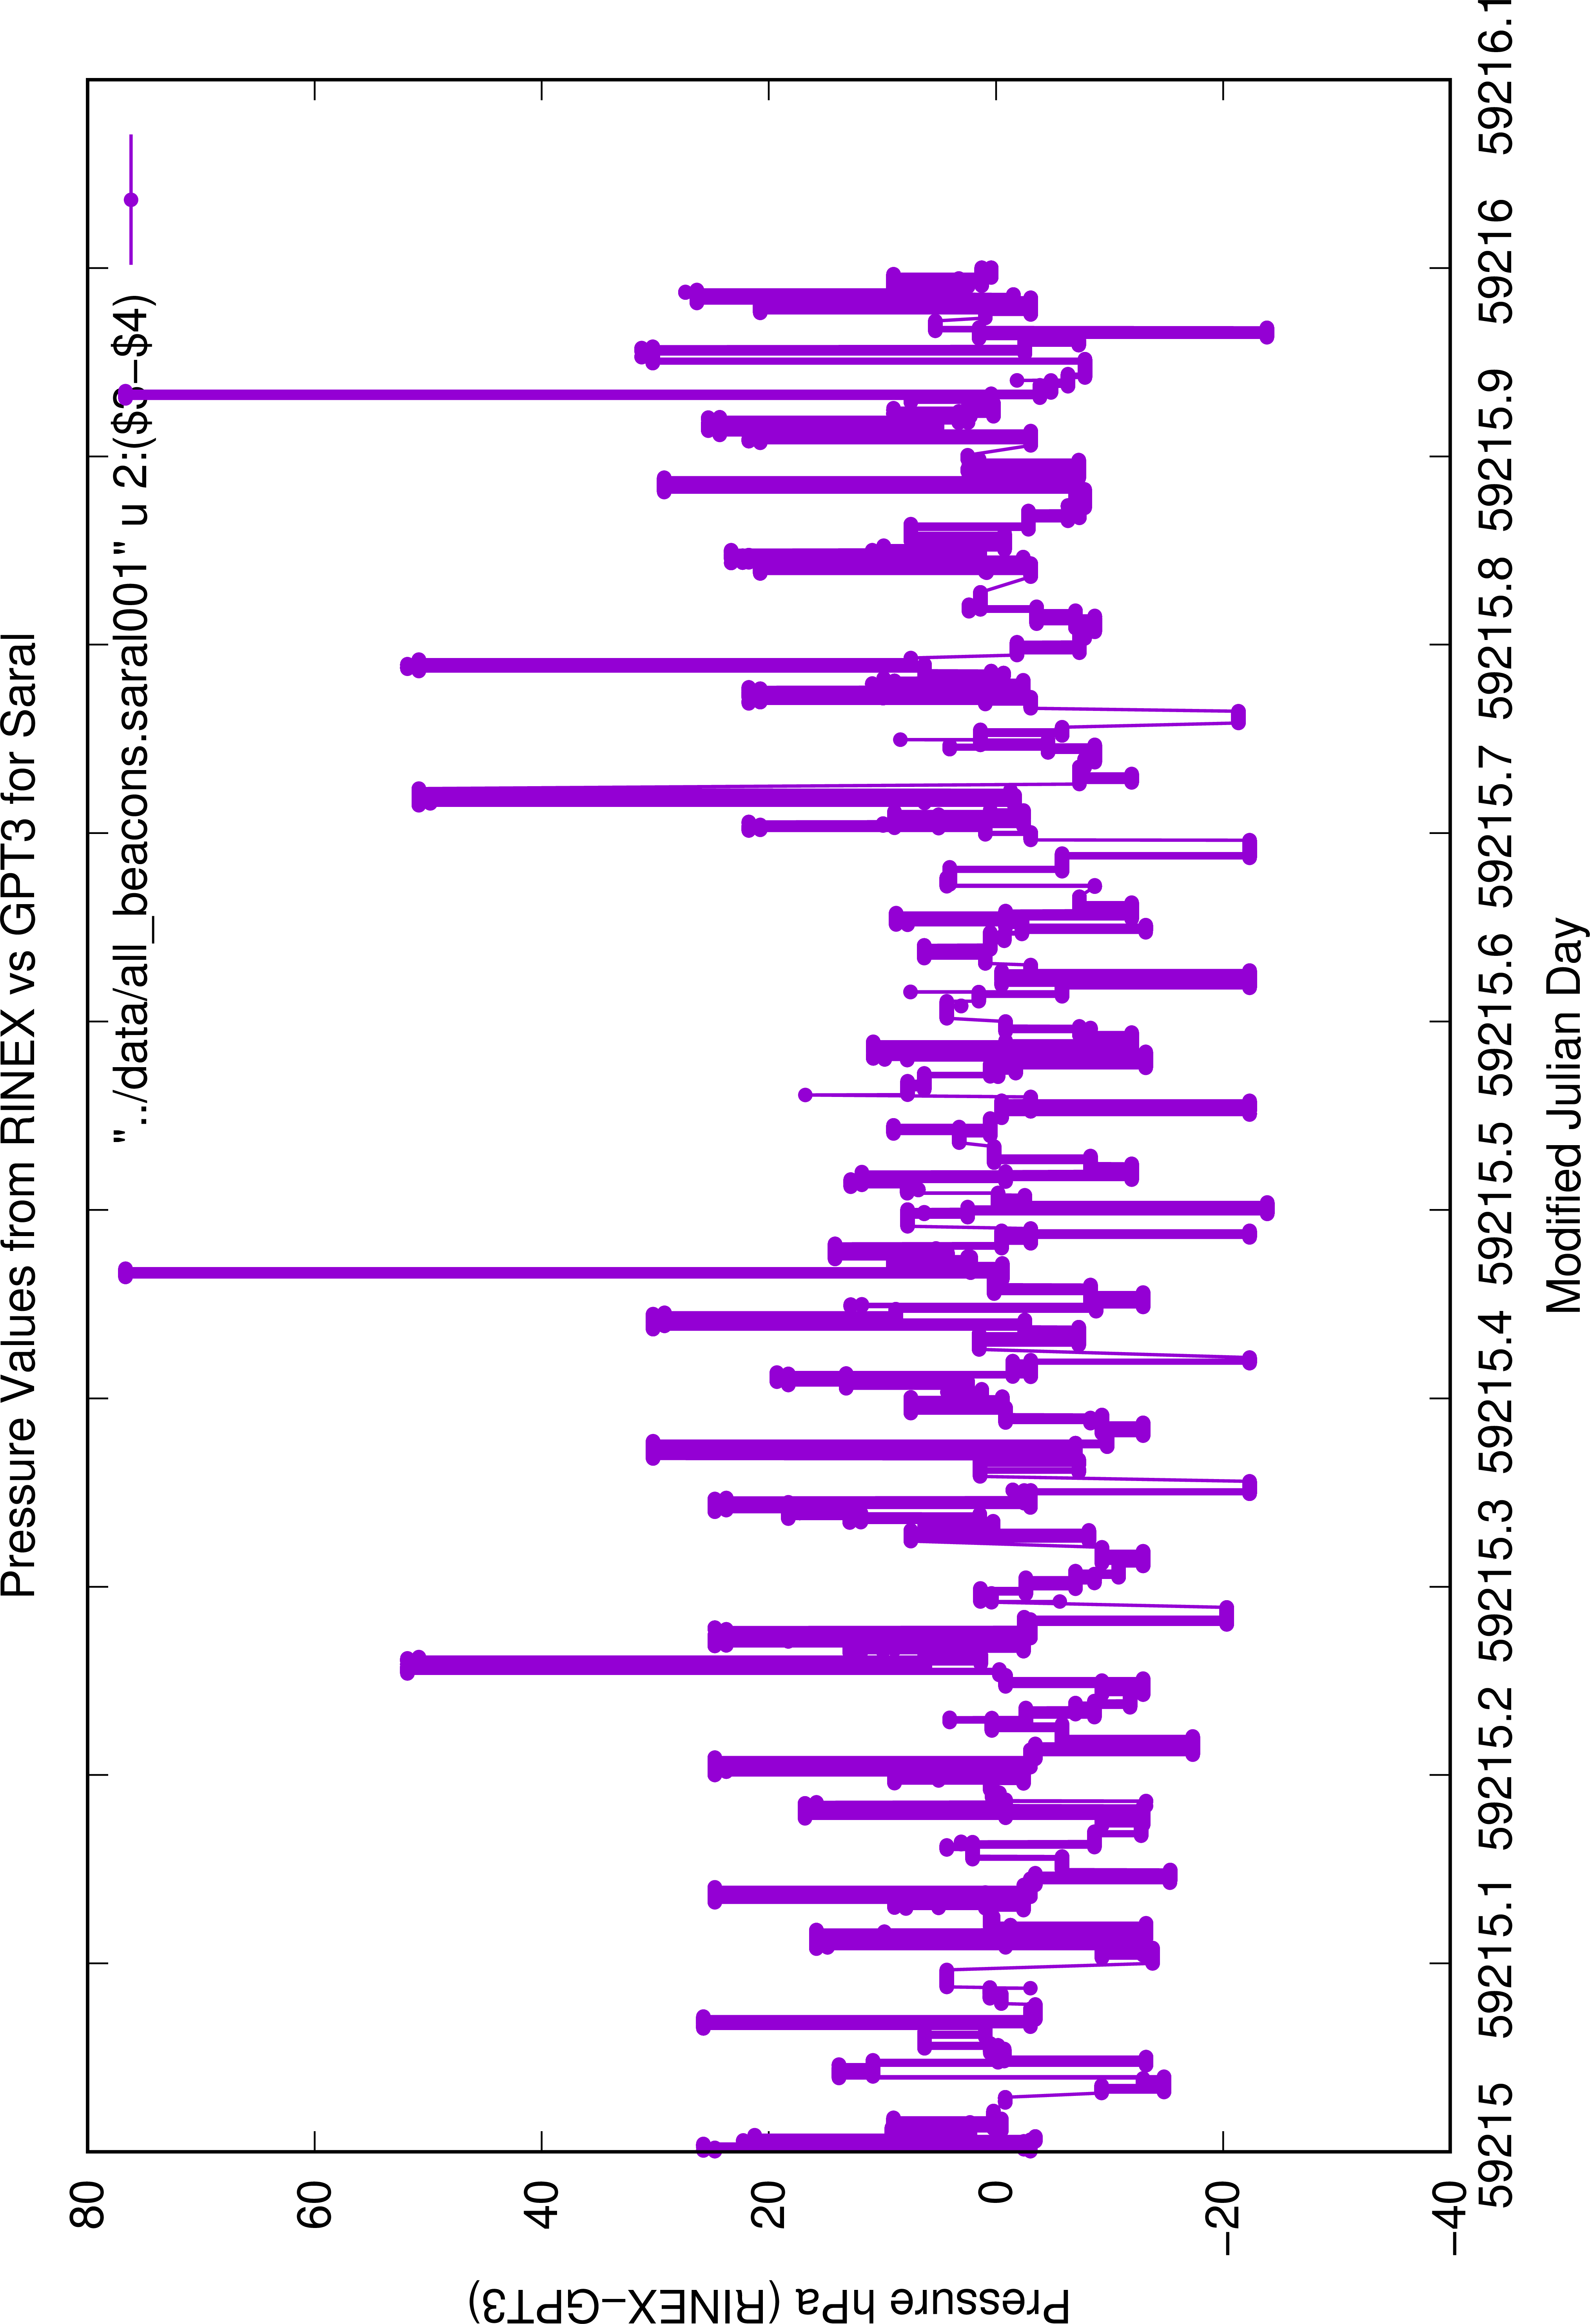
\includegraphics[angle=-90, width=0.5\textwidth]{Saral-allbeacons-pressure}%
    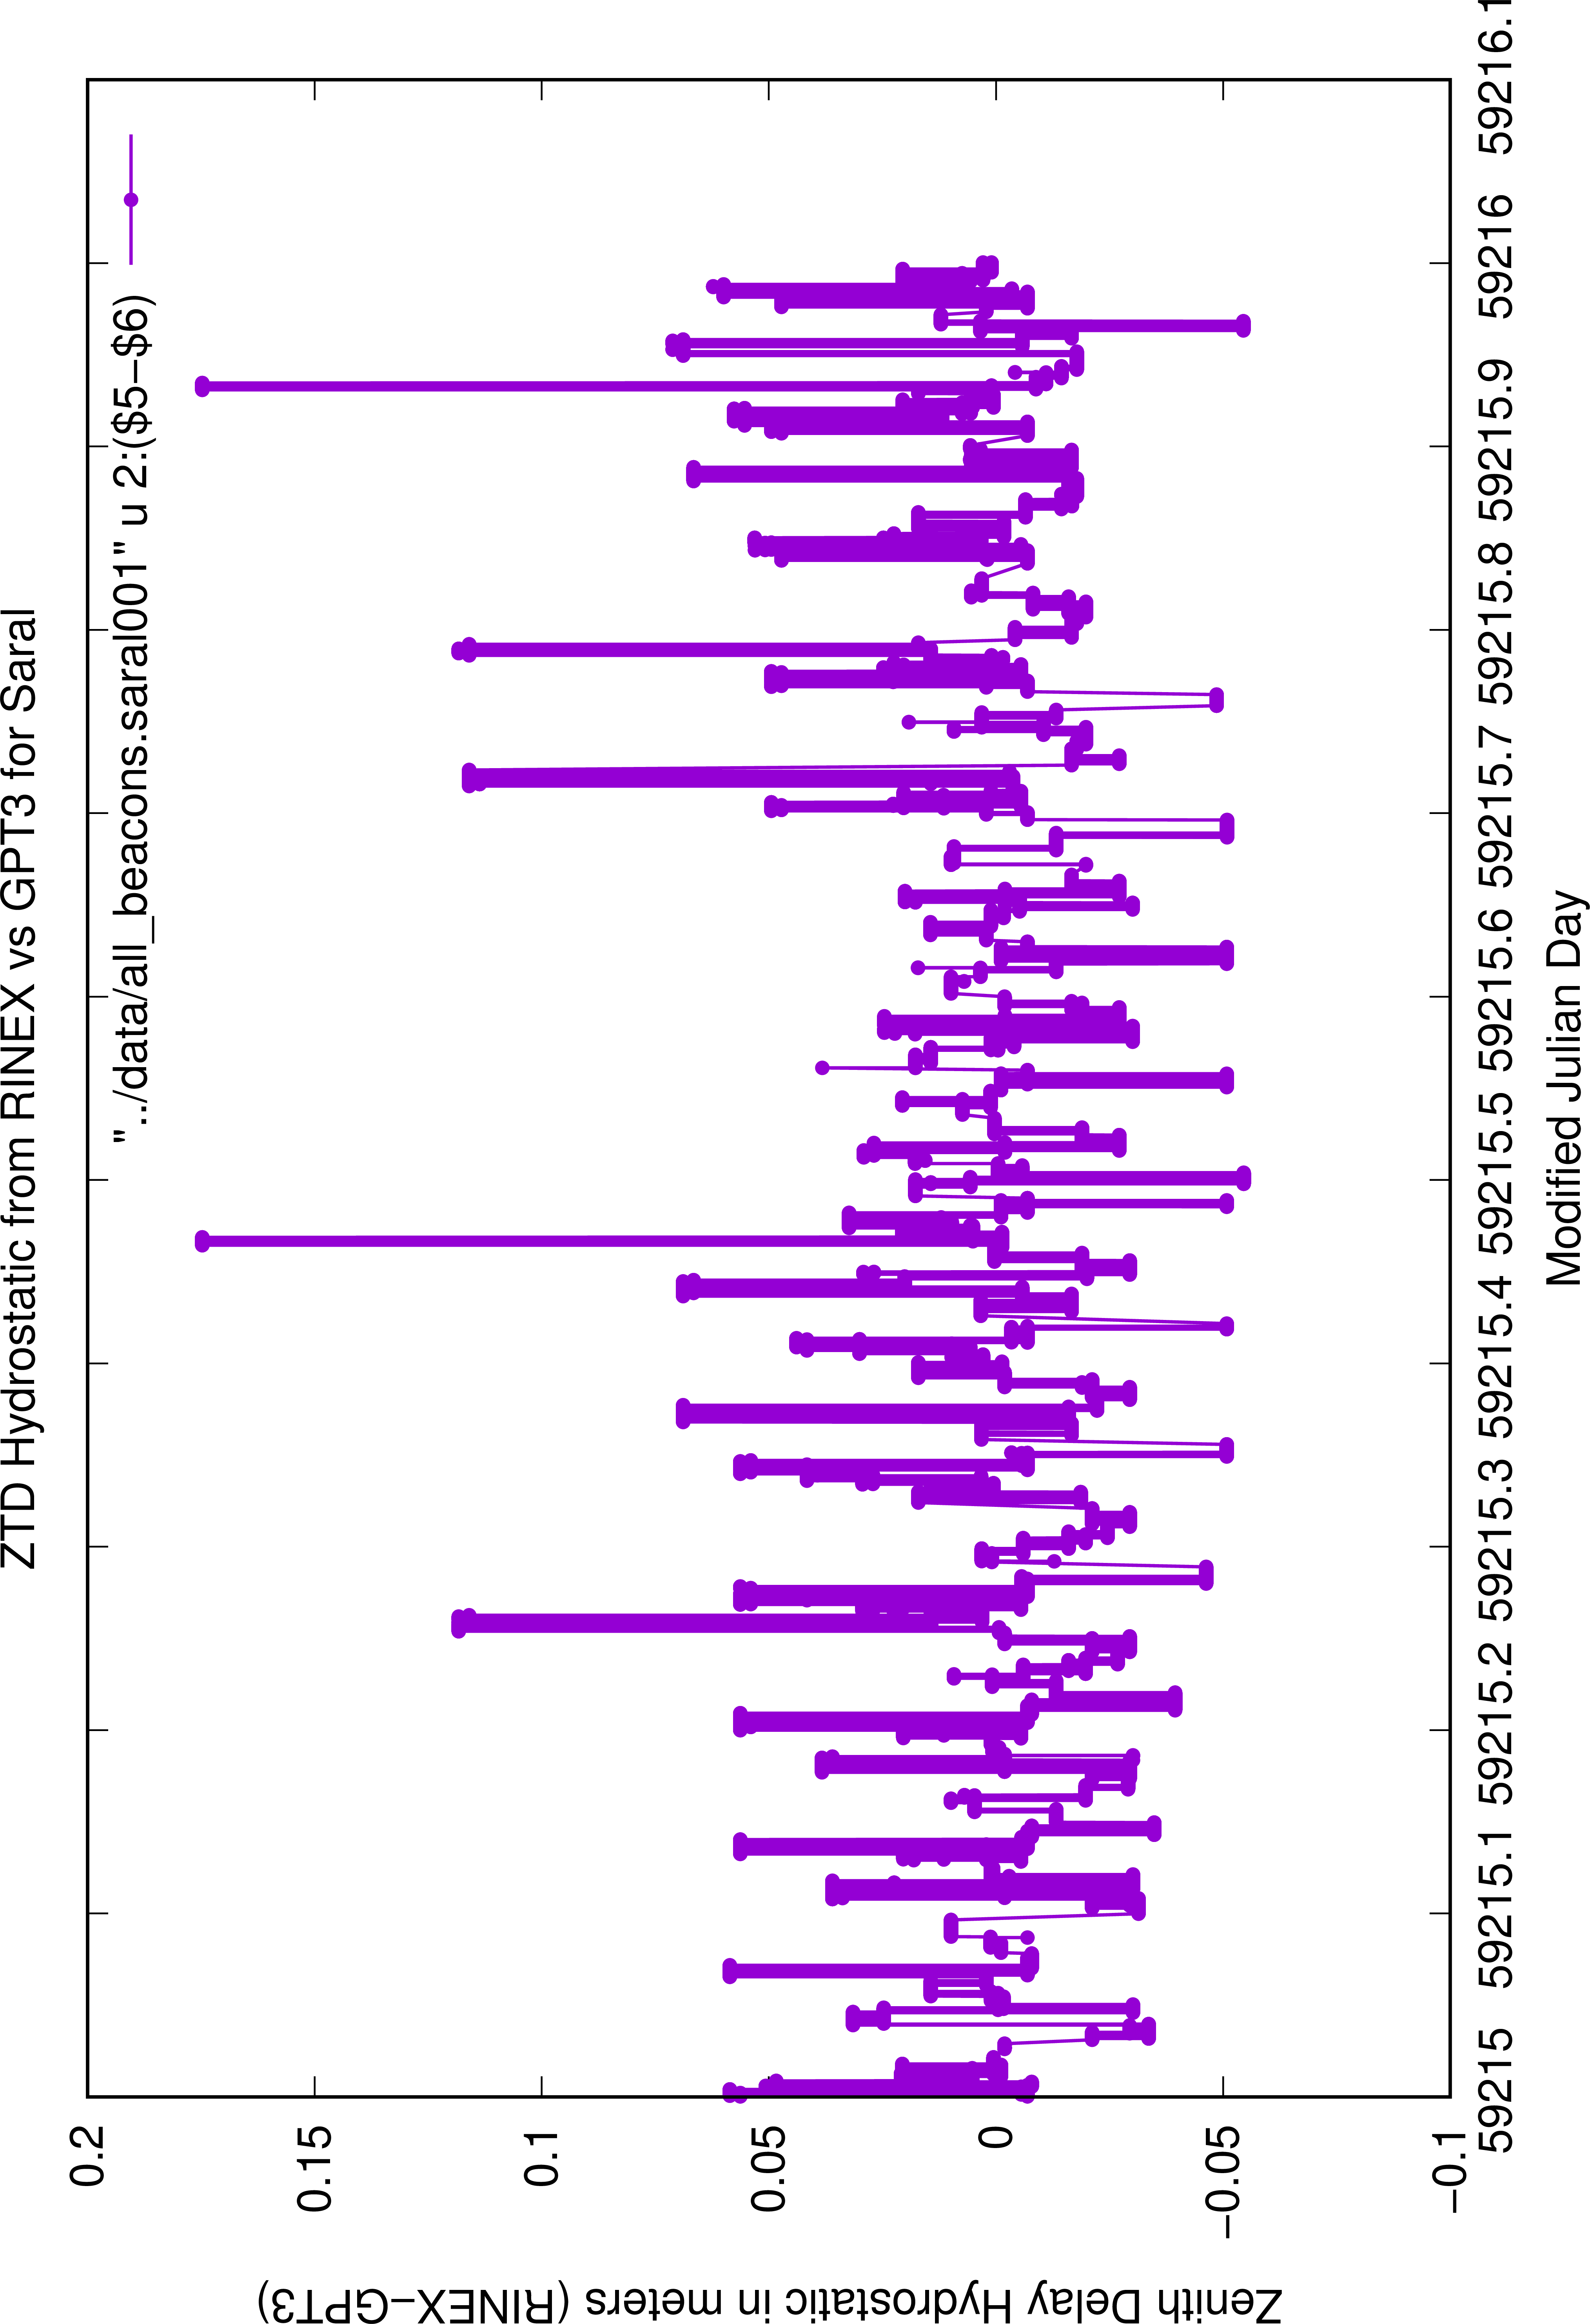
\includegraphics[angle=-90, width=0.5\textwidth]{Saral-allbeacons-ztdh}
  %\end{center}
\end{frame}

\begin{frame}\frametitle{Parameters}\framesubtitle{Tropospheric Delay \(\Delta u_{TROPO}\) (4/)}
  One week of Saral data; Pressure (hPa) and \(ZTD_H\) (m) from RINEX Vs GPT3 derived values for beacon TLSB (France)
  %\begin{center}
    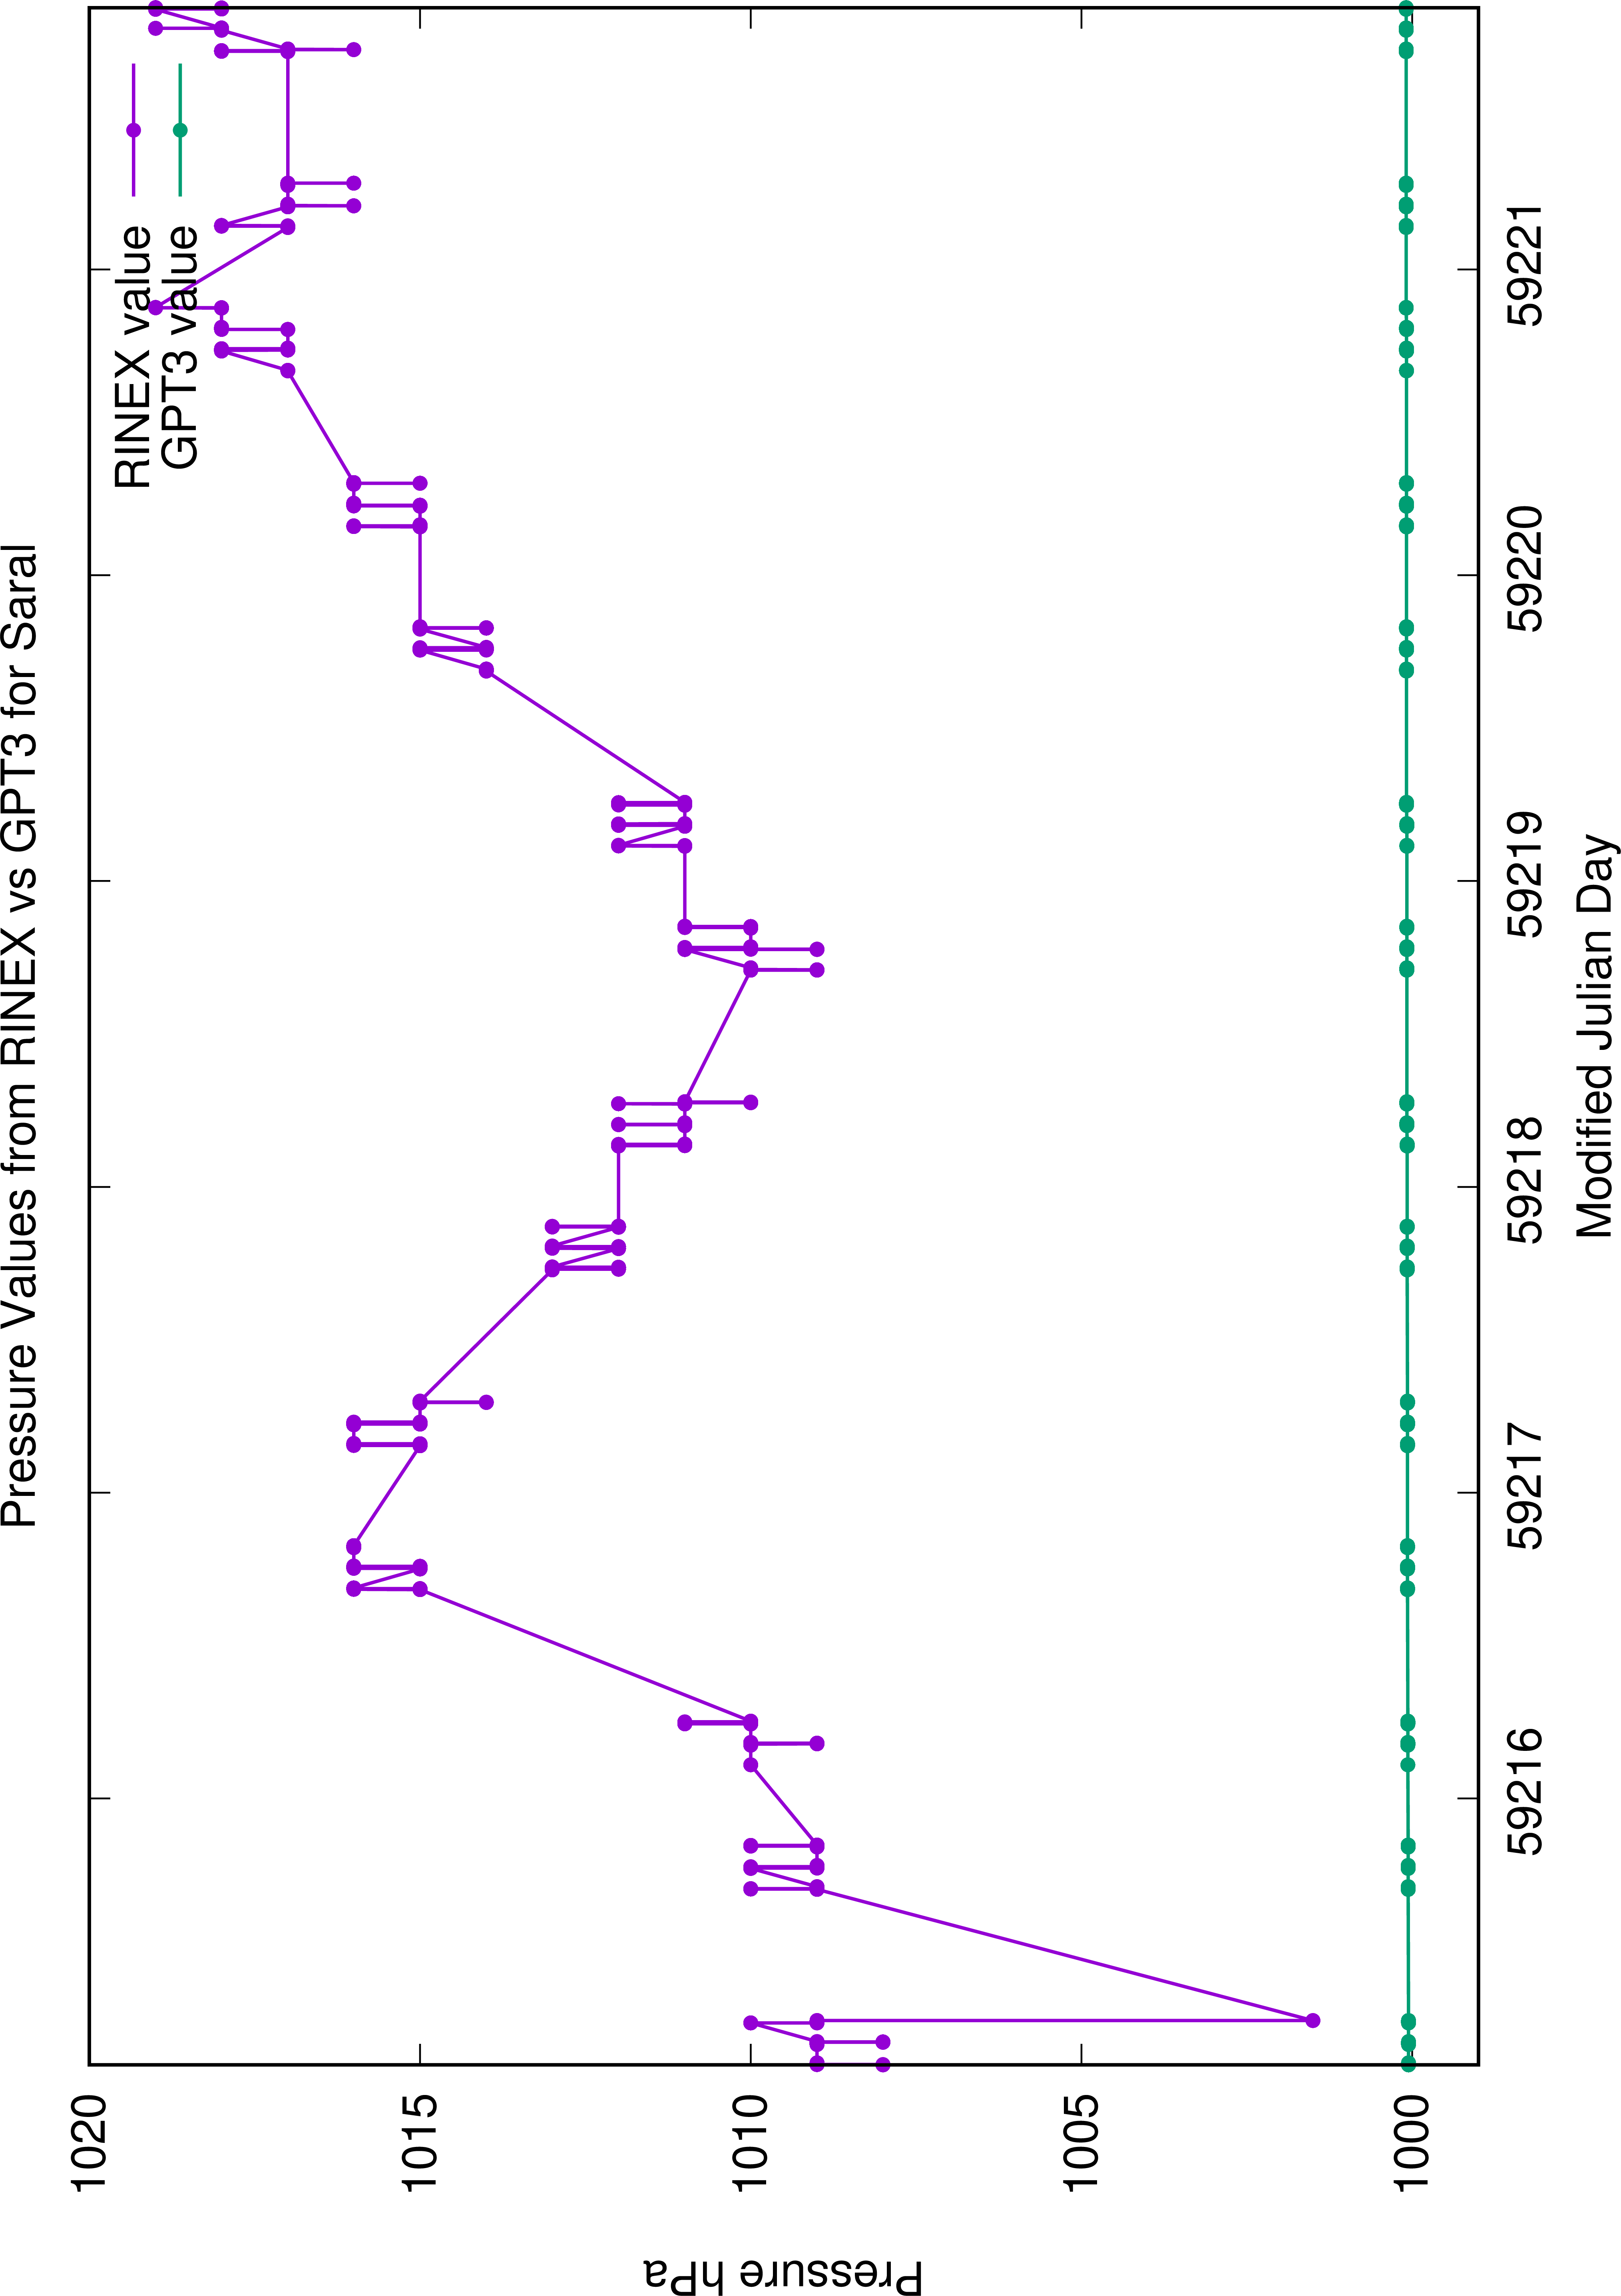
\includegraphics[angle=-90, width=0.5\textwidth]{Saral-TLSB-pressure12}%
    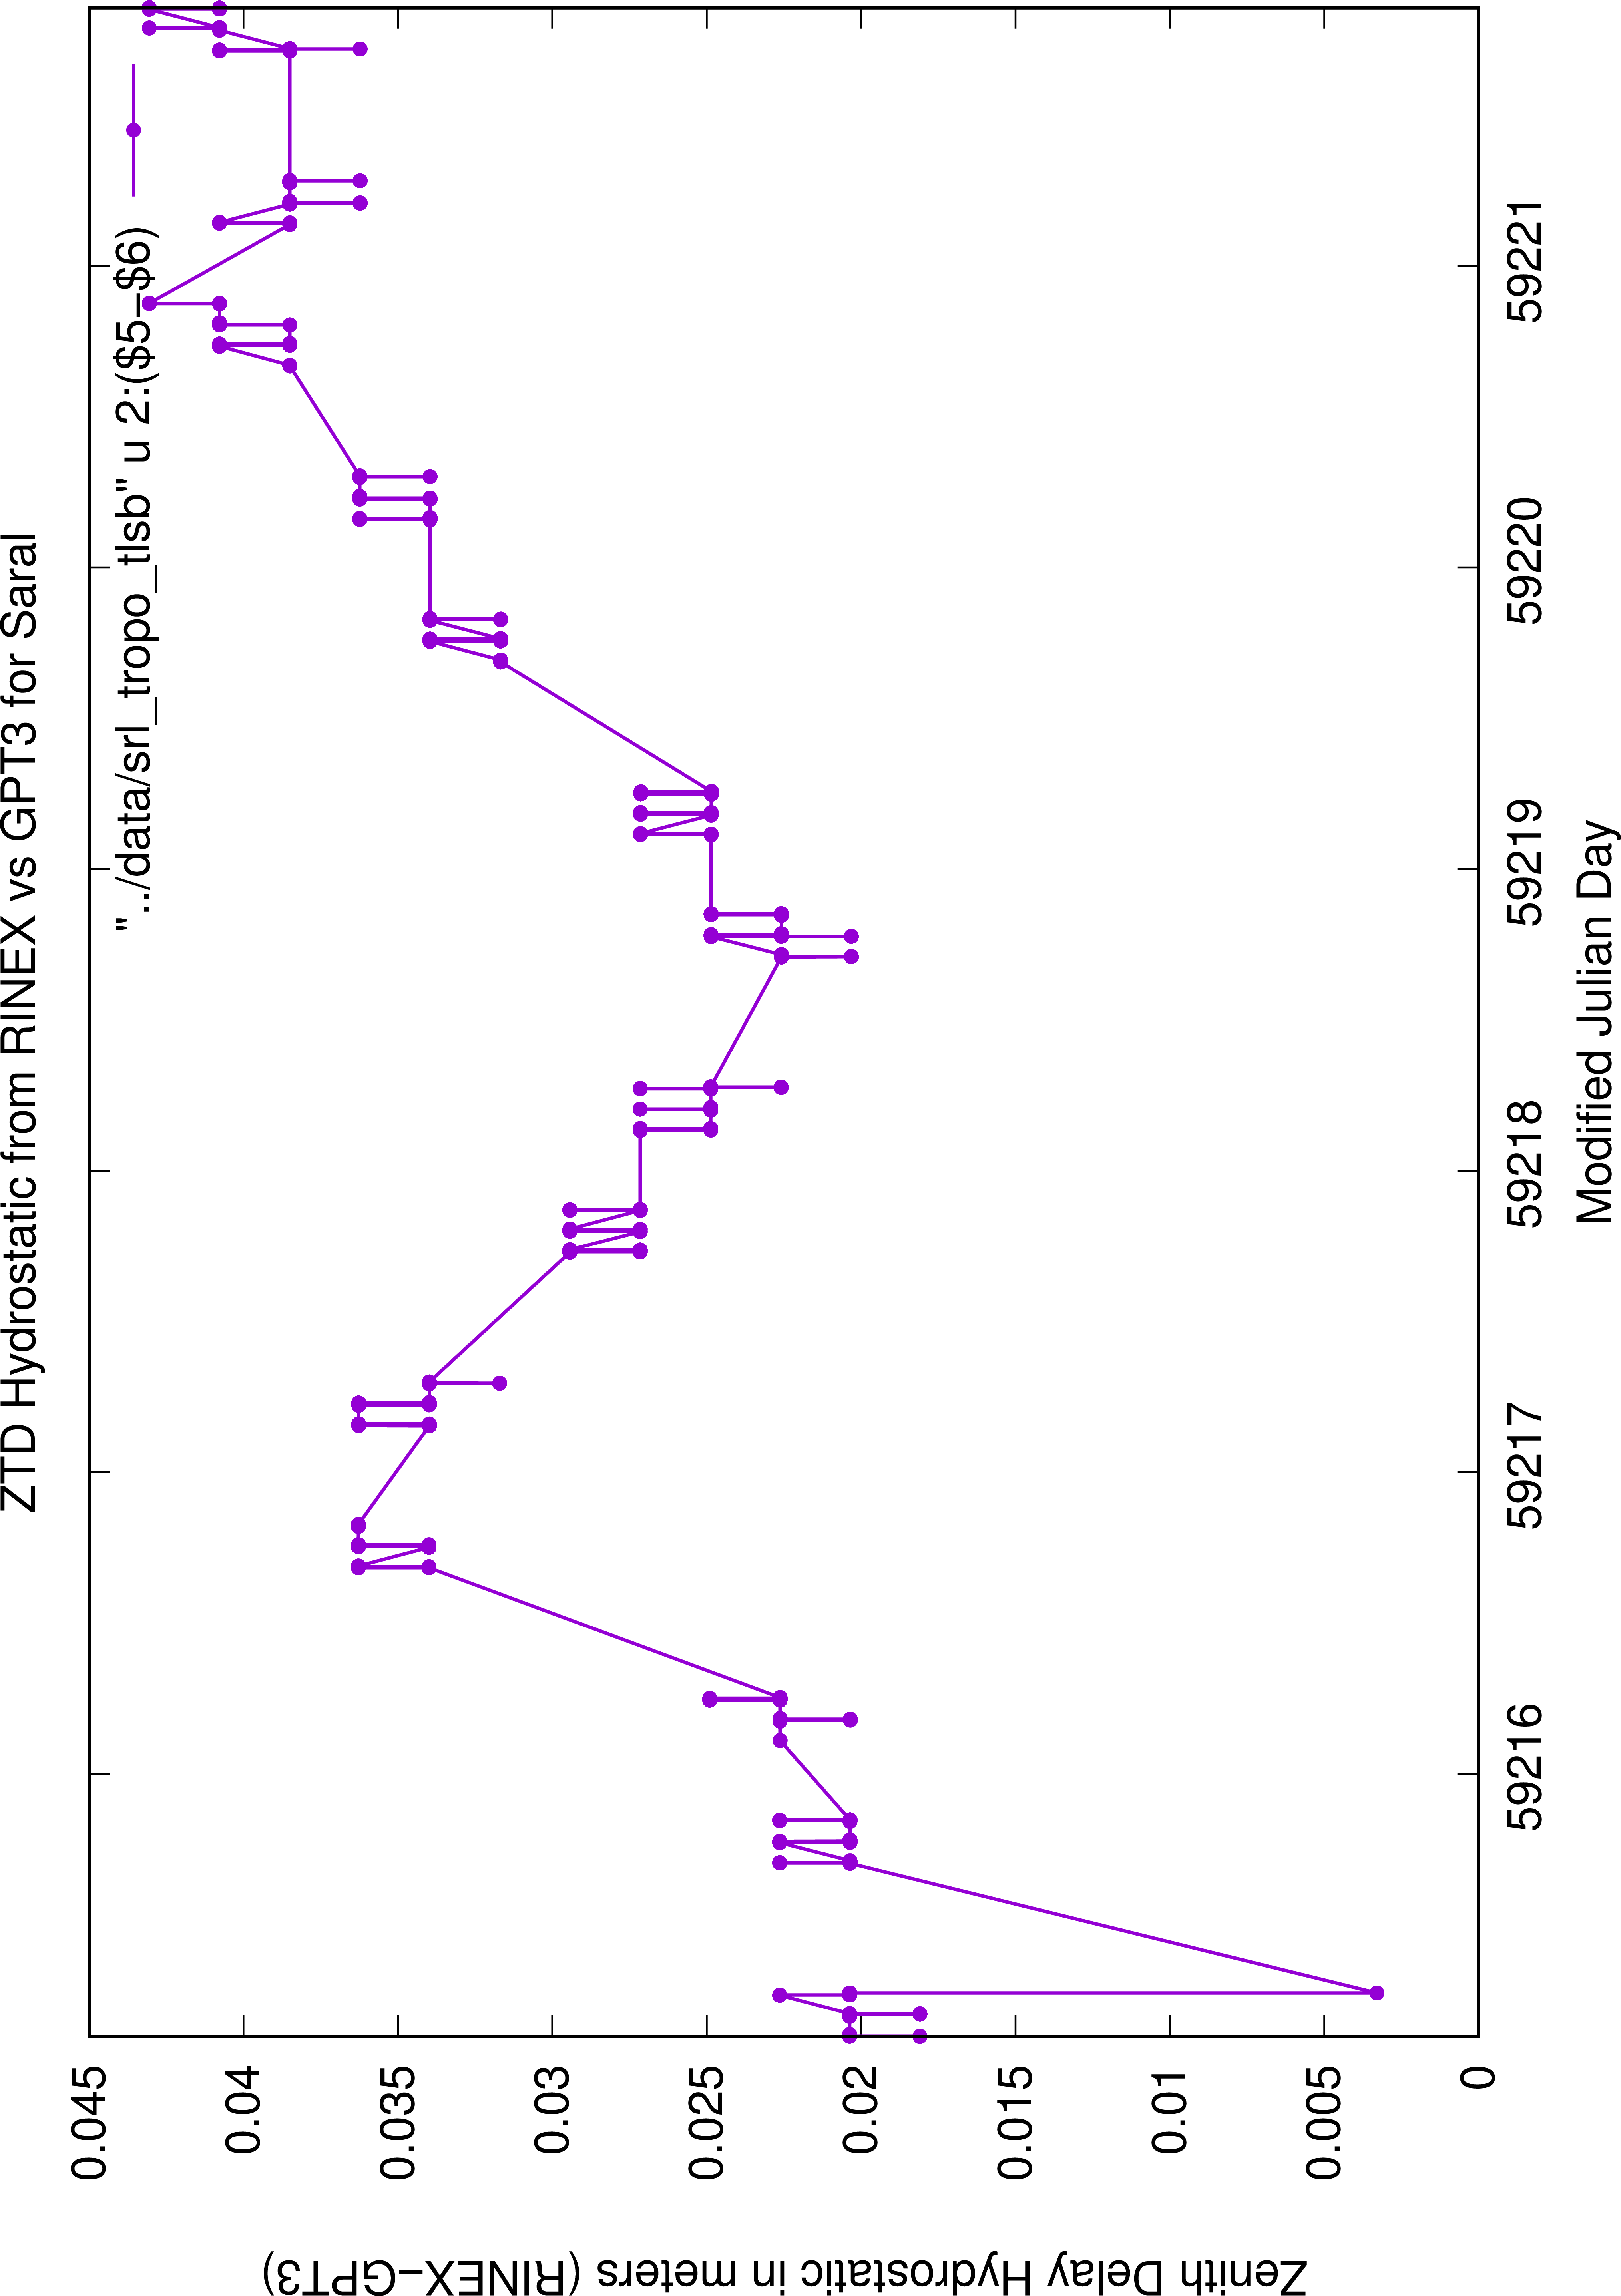
\includegraphics[angle=-90, width=0.5\textwidth]{Saral-TLSB-ztdh}
    \begin{tikzpicture}[overlay, remember picture] 
      \node at (current page.north east) 
          [
          anchor=north east,
          xshift=-3cm,
          yshift=-7cm
          ] 
      {
      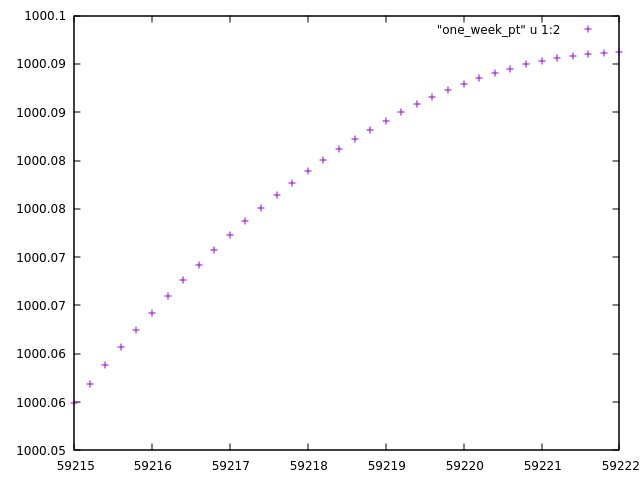
\includegraphics[width=0.3\textwidth]{gpt3_pressure_one_week}
      };
      \end{tikzpicture}
  %\end{center}
\end{frame}

\begin{frame}\frametitle{Parameters}\framesubtitle{Tropospheric Delay \(\Delta u_{TROPO}\) (5/)}
  Elevation Vs Total tropospheric delay; SV: Saral, orbital period = 100.6 minutes
  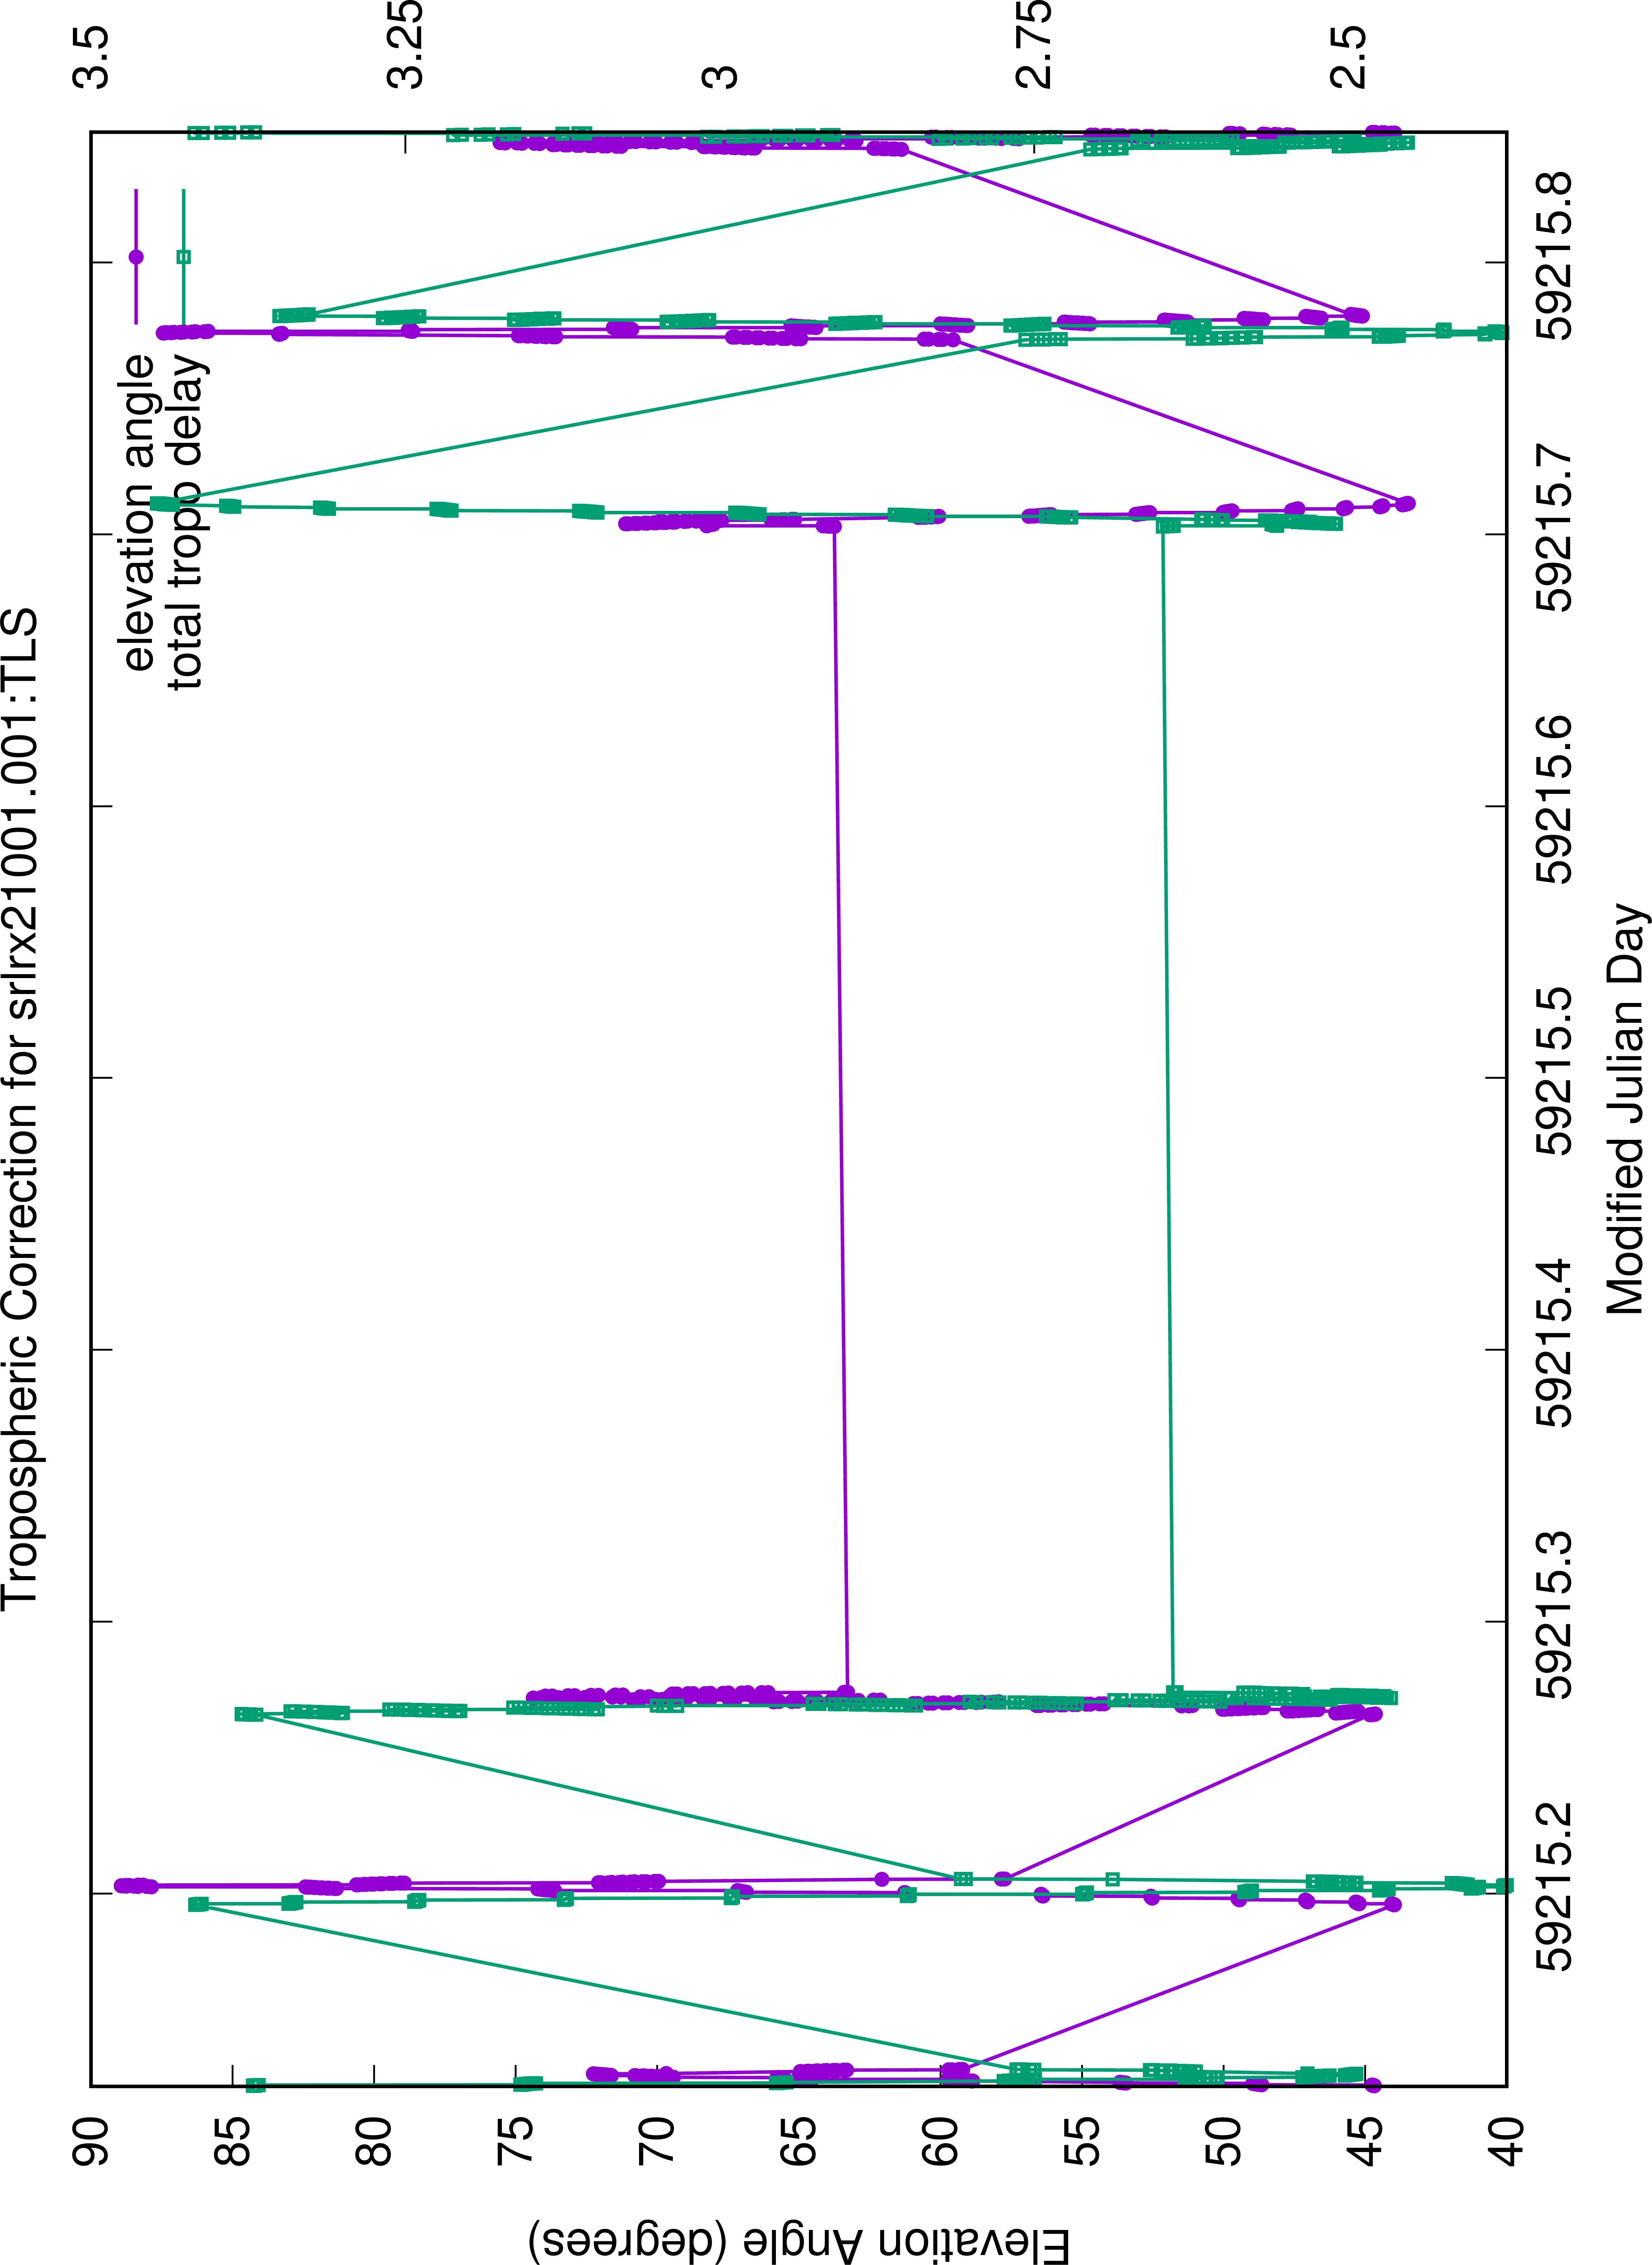
\includegraphics[angle=-90, width=0.9\textwidth]{srlrx21001.001-tropo-correction-one-day}%
  \begin{tikzpicture}[overlay, remember picture] 
    \node at (current page.north east) 
        [
        anchor=north east,
        xshift=-4cm,
        yshift=-3cm
        ] 
    {
    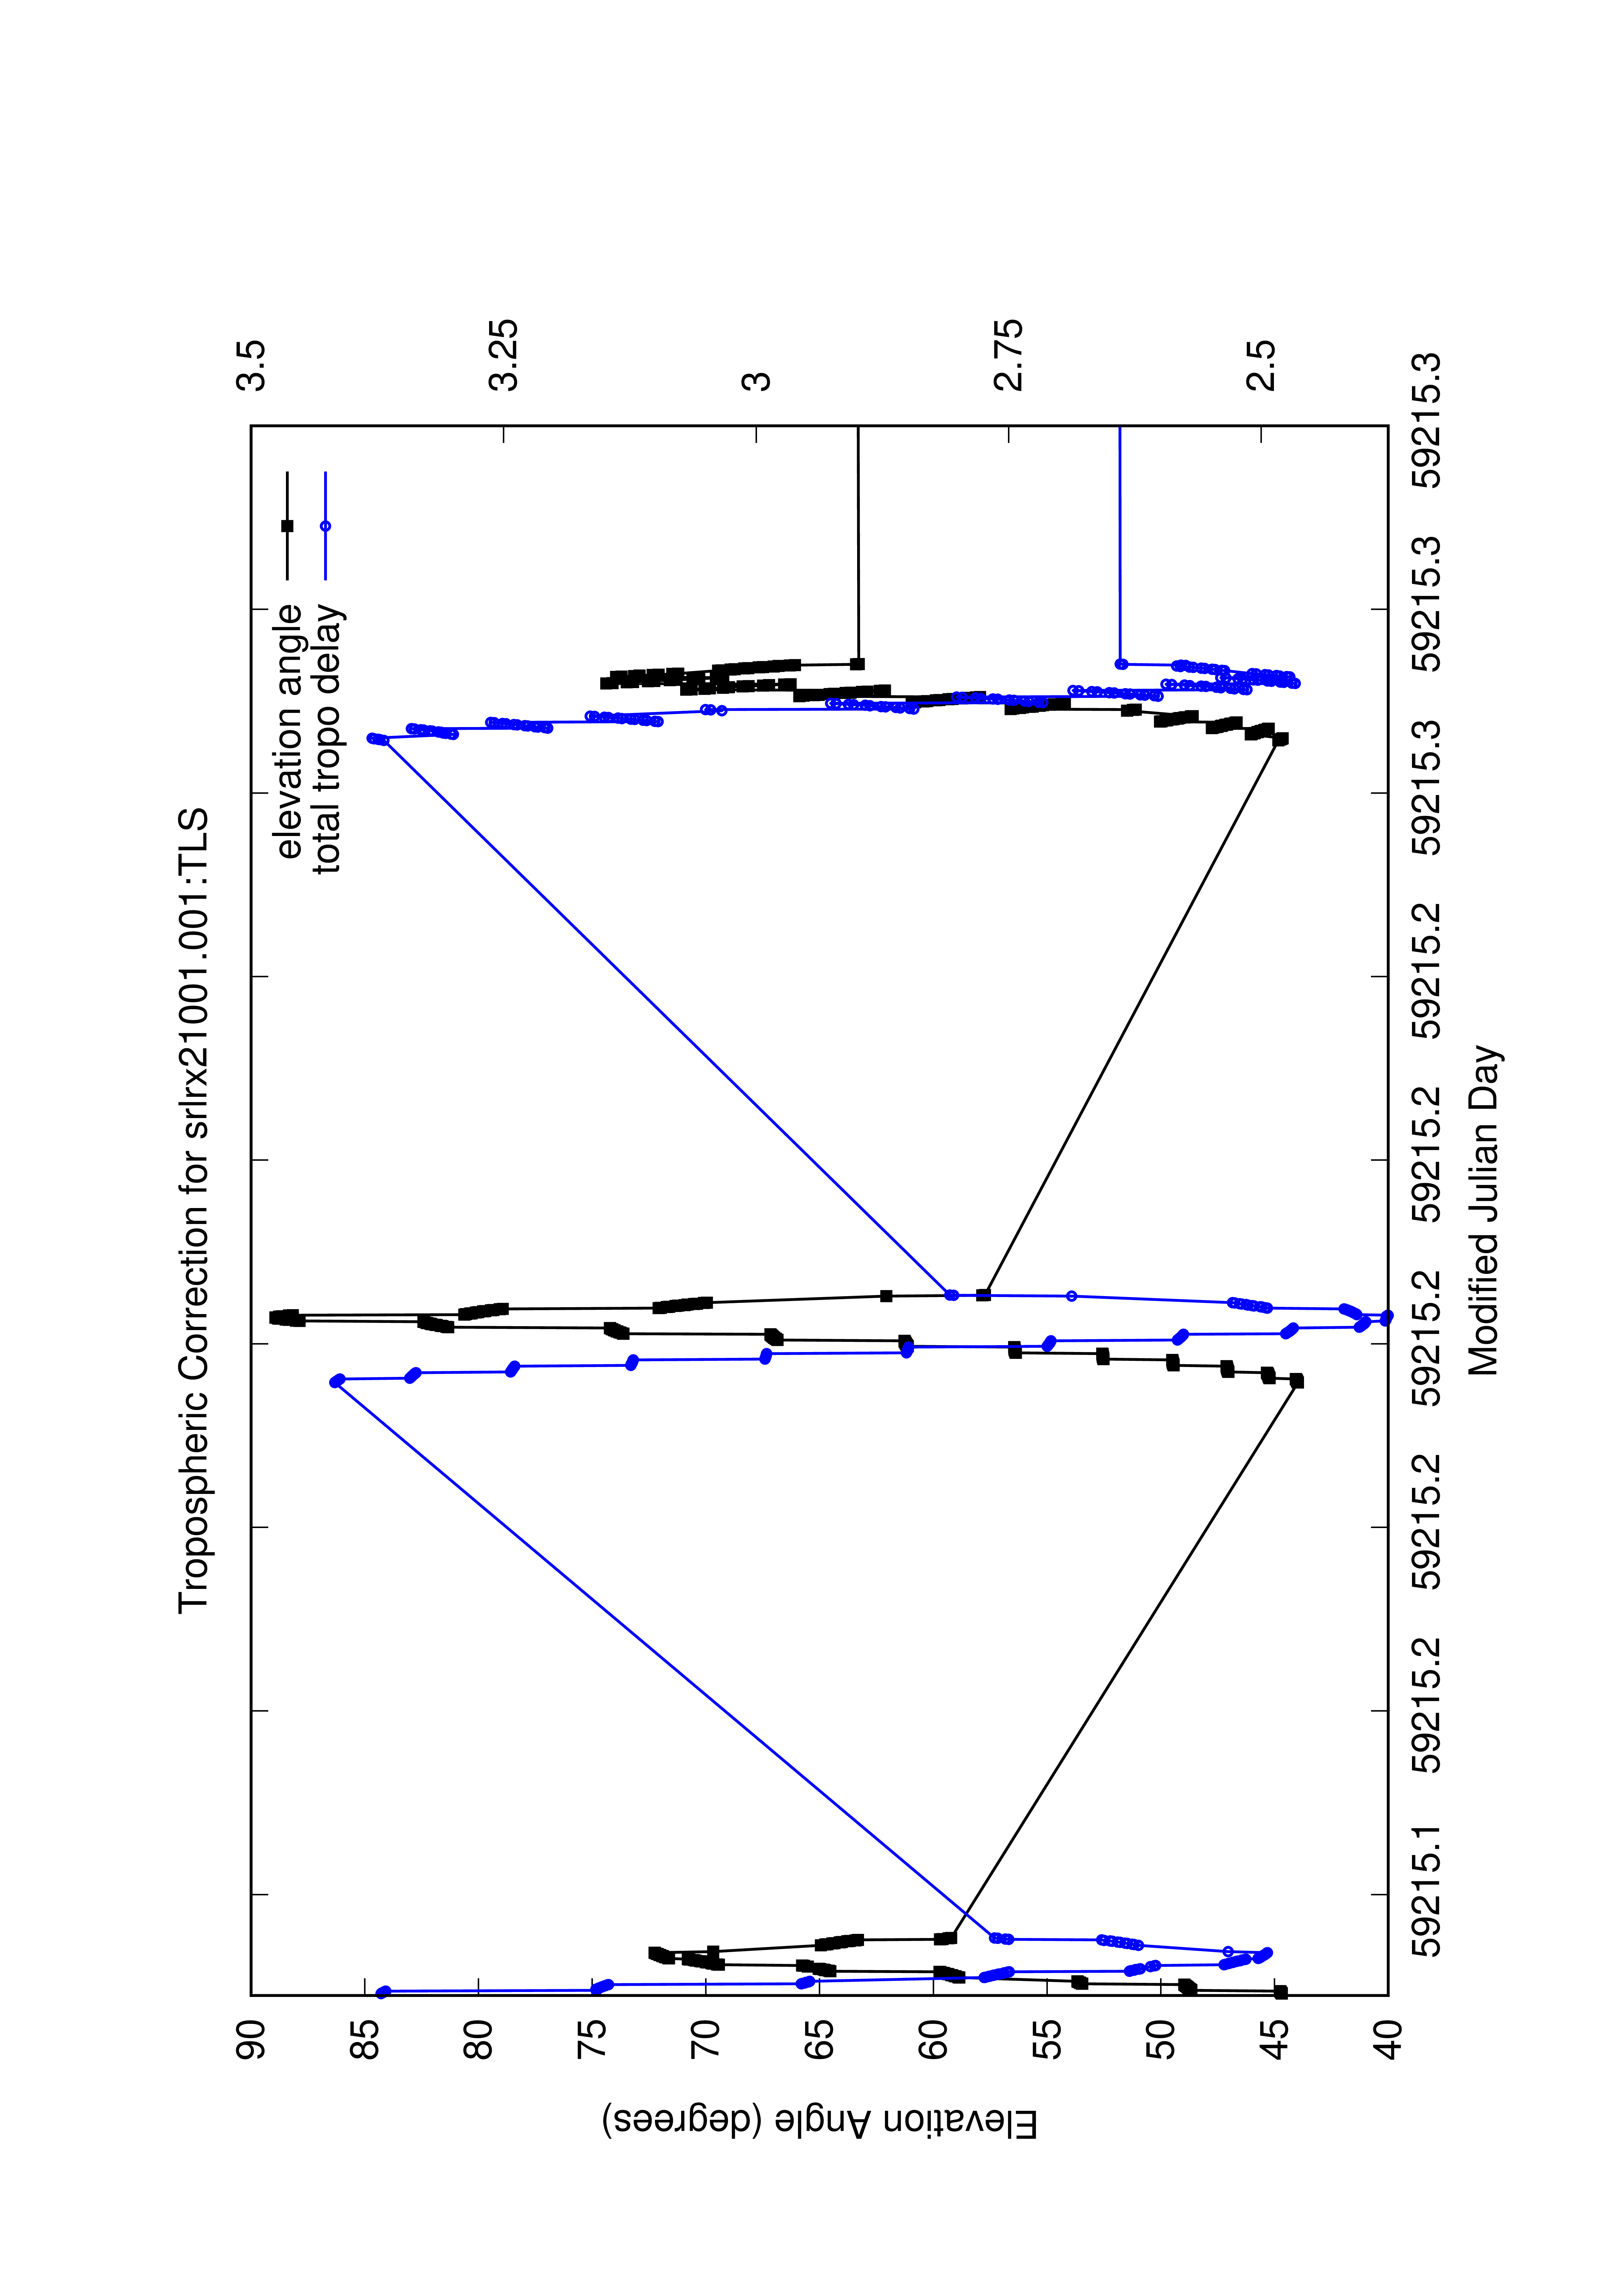
\includegraphics[angle=-90, width=0.5\textwidth]{srlrx21001.001-tropo-correction-half-day}
    };
    \end{tikzpicture}
\end{frame}

\begin{frame}\frametitle{Parameters}\framesubtitle{Tropospheric Delay \(\Delta u_{TROPO}\) (6/)}
  Elevation Vs Total tropospheric delay; SV: Sentinel-6A, orbital period =  minutes
  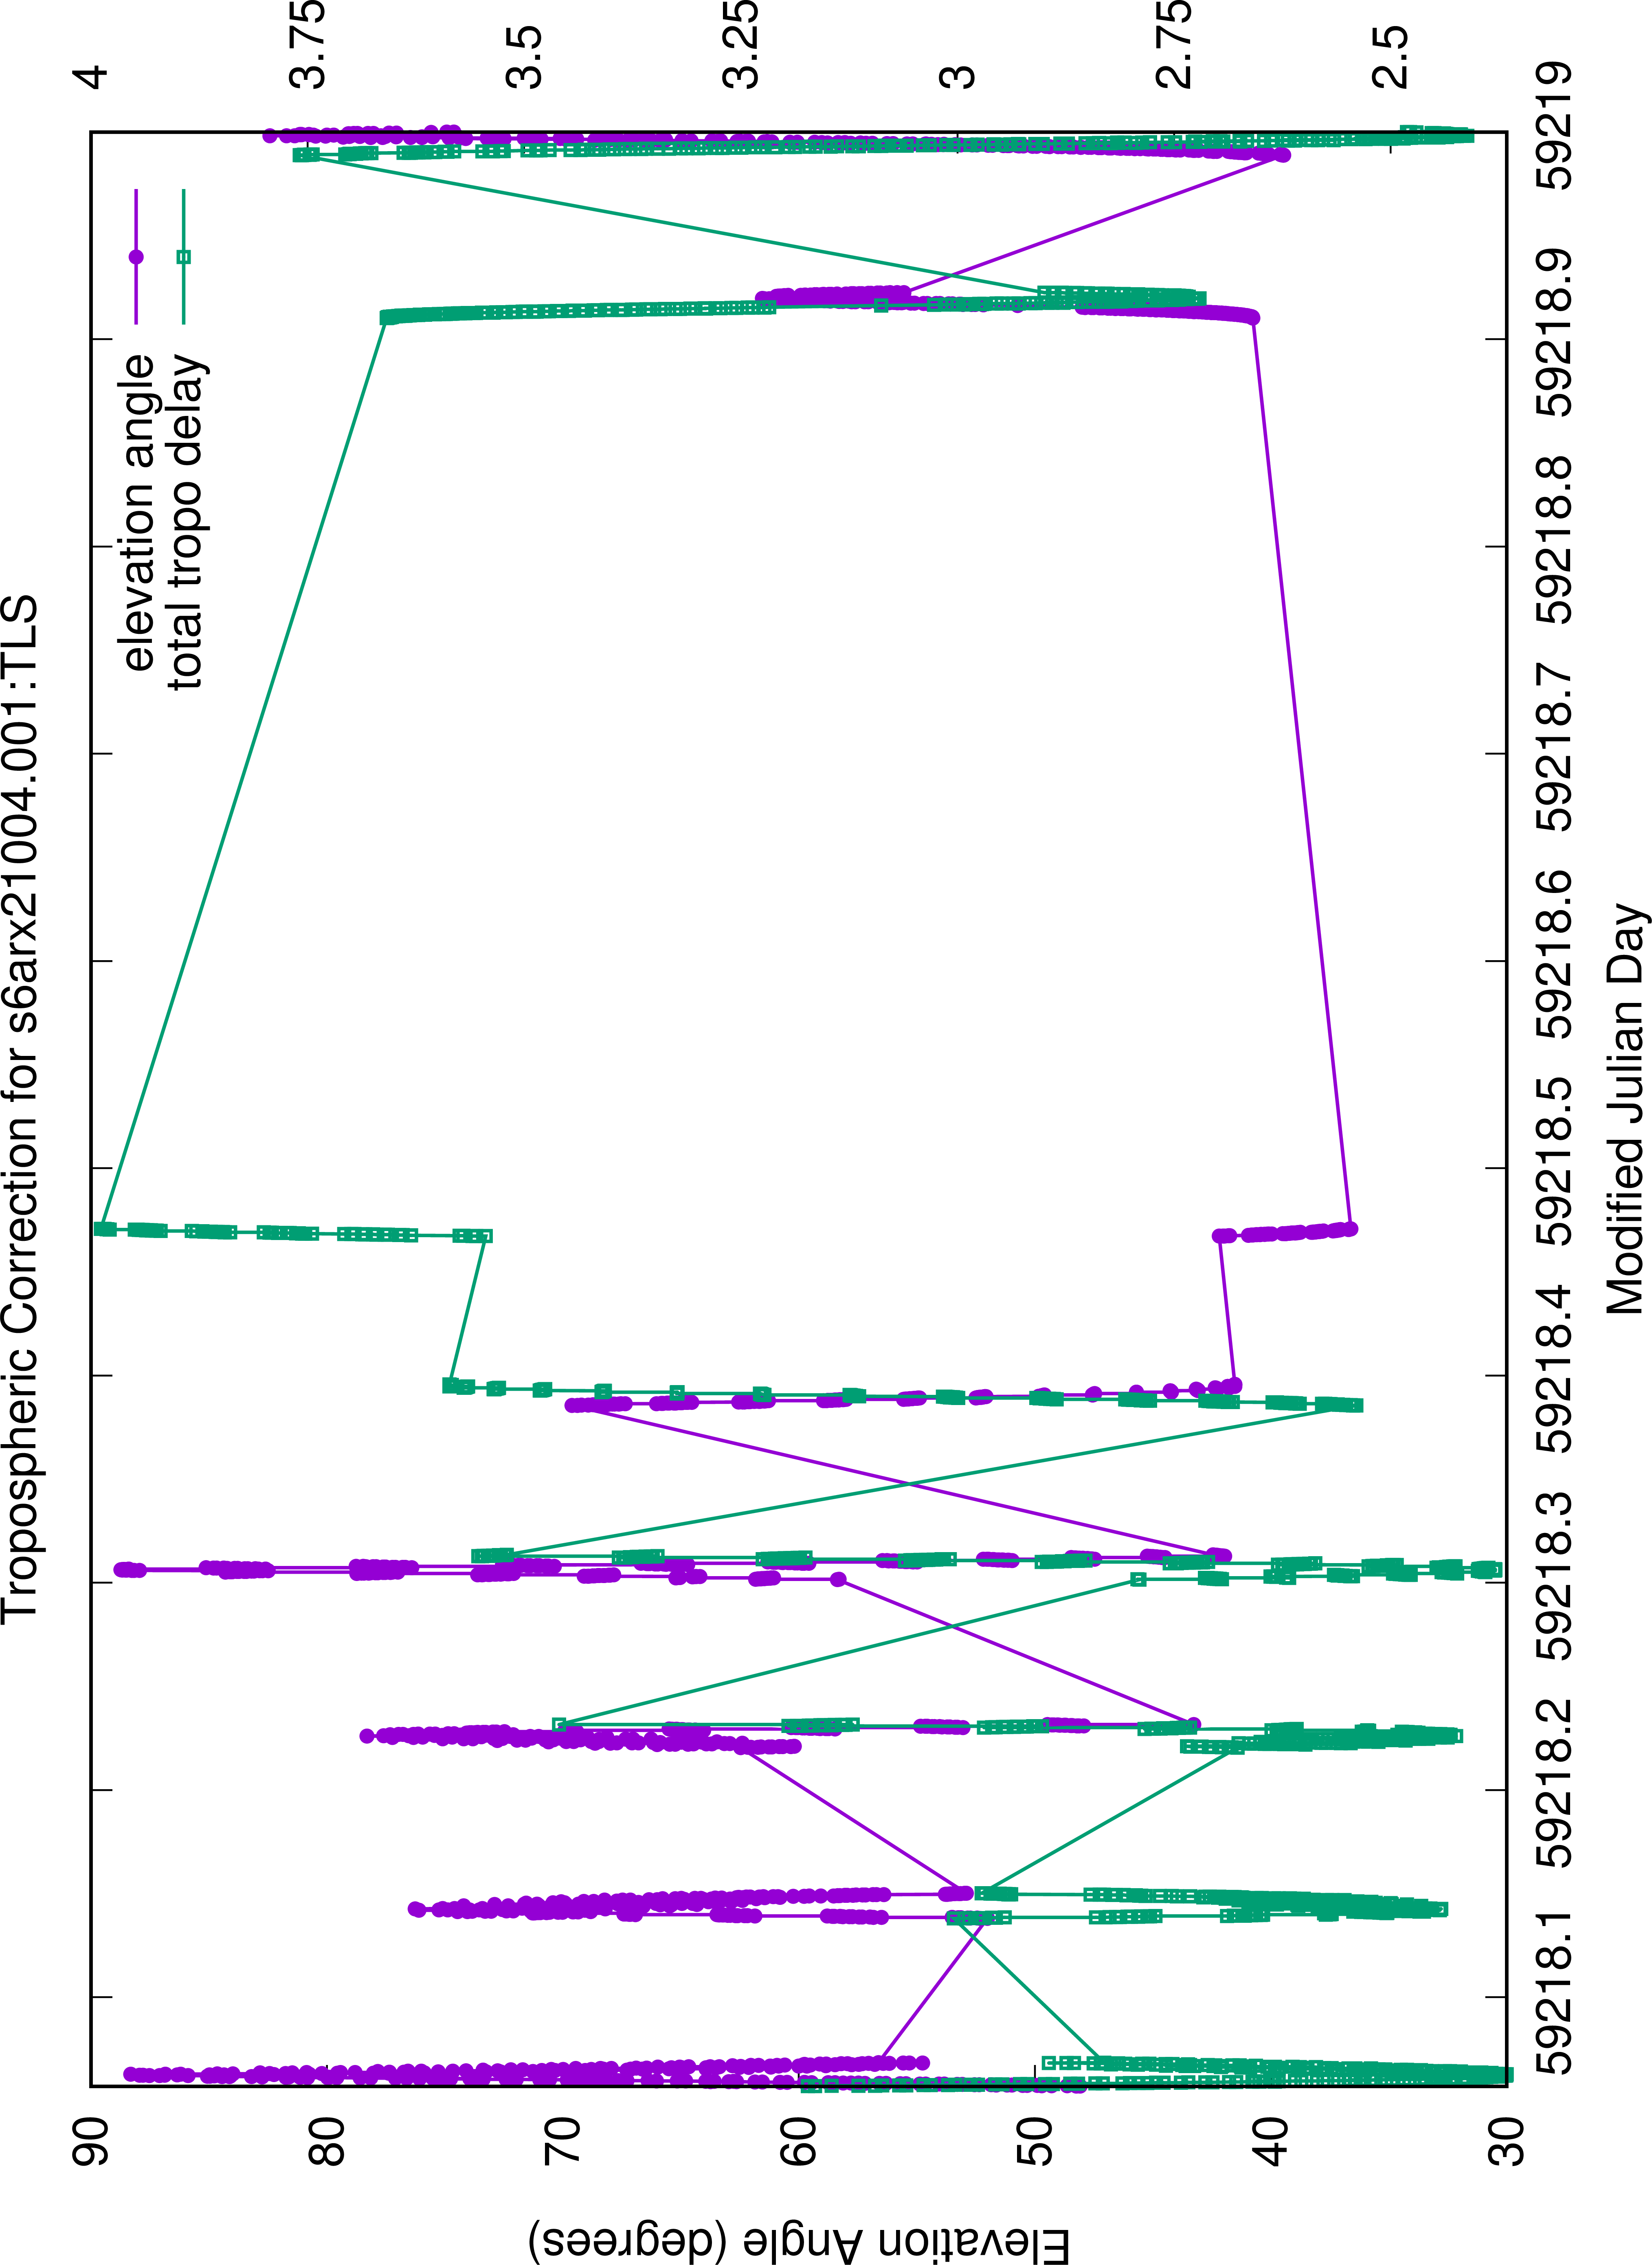
\includegraphics[angle=-90, width=0.85\textwidth]{s6arx21004.001-tropo-correction-one-day.png}%
  \begin{tikzpicture}[overlay, remember picture] 
    \node at (current page.north east) 
        [
        anchor=north east,
        xshift=-2.5cm,
        yshift=-3cm
        ]
    {
    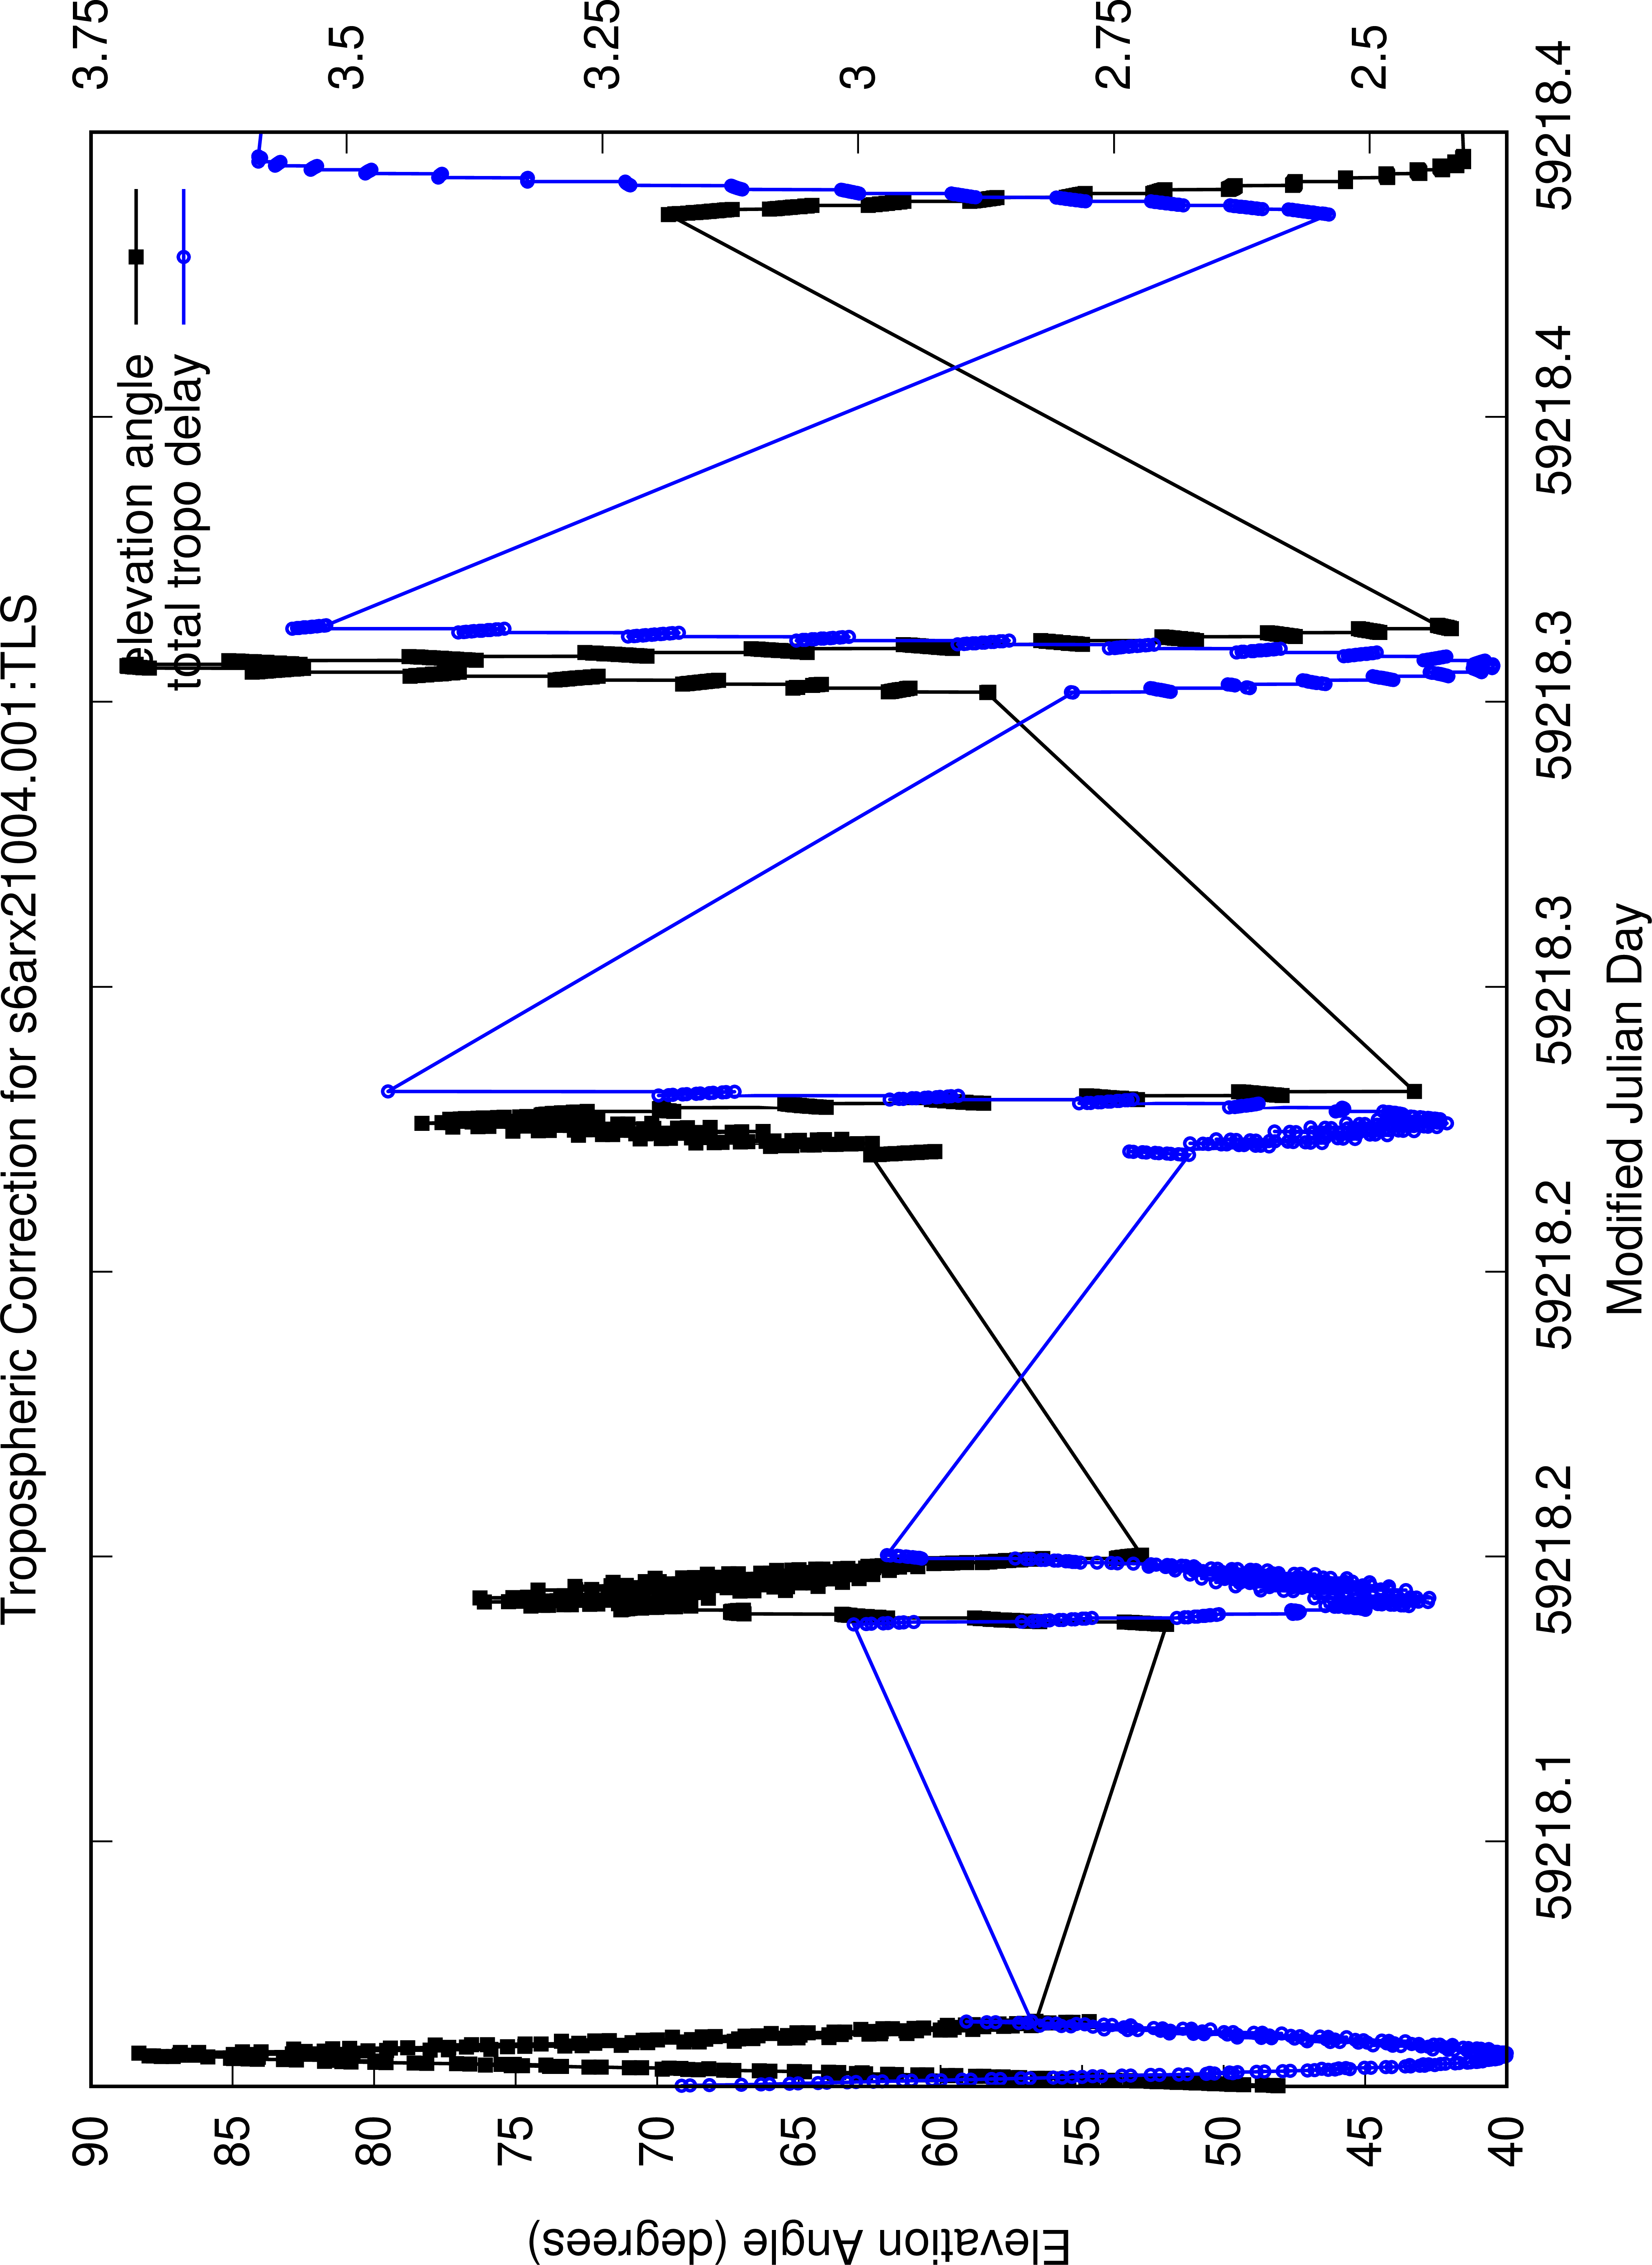
\includegraphics[angle=-90, width=0.5\textwidth]{s6arx21004.001-tropo-correction-half-day.png}
    };
    \end{tikzpicture}
\end{frame}

\begin{frame}\frametitle{Parameters}\framesubtitle{Tropospheric Delay \(\Delta u_{TROPO}\) (7/)}
  Elevation Vs Total tropospheric delay; SV: Cryosat, orbital period = 99.16 minutes
  \begin{center}
  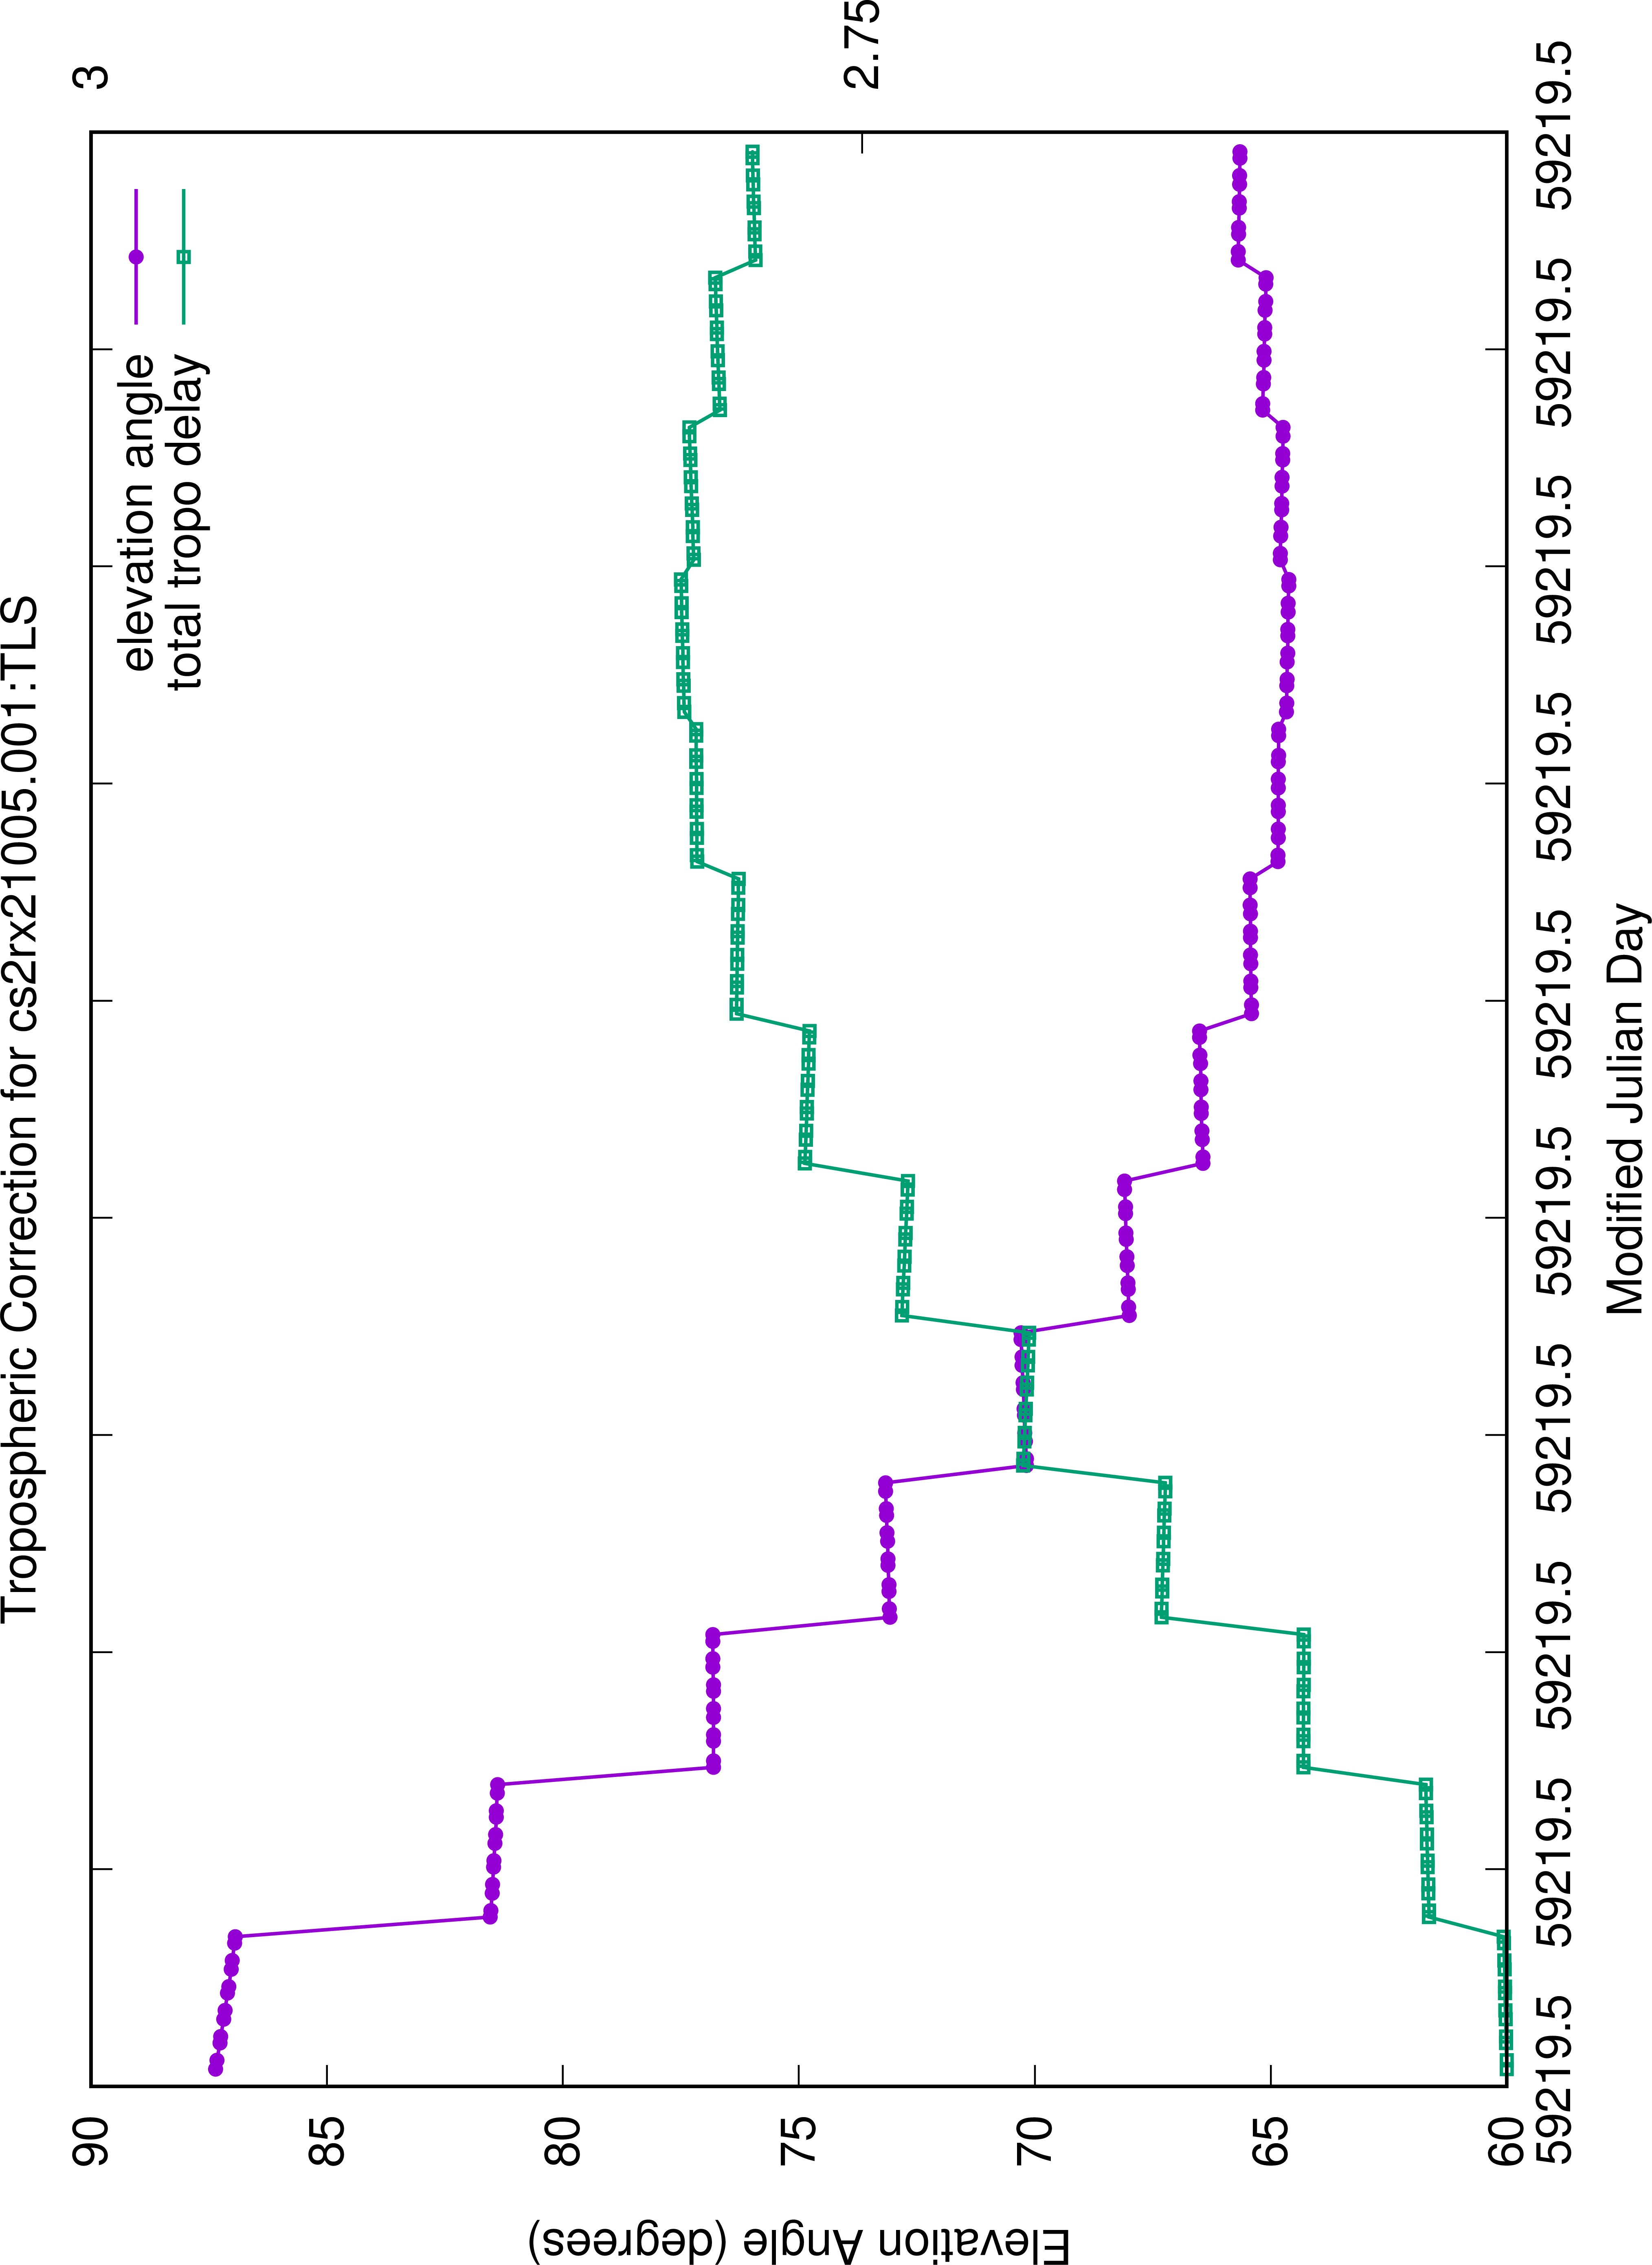
\includegraphics[angle=-90, width=0.8\textwidth]{cs2rx21005.001-tropo-correction}
  \end{center}
\end{frame}

\begin{frame}\frametitle{Parameters}\framesubtitle{Tropospheric Delay \(\Delta u_{TROPO}\) (8/)}
  \textcolor{red}{Todo:}
  \begin{itemize}
    %\bitem use the more precise \(1 \degree \times 1 \degree \) gpt3 grid (currently using the \(5 \degree \times 5 \degree \) version)
    \bitem use the more precise \(1^\circ \times 1^\circ \) gpt3 grid (currently using the \(5^\circ \times 5^\circ \) version)
    \bitem \(ZTD_{wet}\) should be estimated (instead of computed)
    \bitem include gradients (map azimouthal ZTD dependency)
    \bitem use more DORIS-derived measurements (e.g. temperature) to model tropospheric delay
  \end{itemize}
\end{frame}

\begin{frame}\frametitle{Parameters}\framesubtitle{Ionospheric Delay \(\Delta u_{IONO}\) (1/)}
  \begin{equation*}
    \left.\begin{aligned}
        u_{measured} & = \frac{\color{red}c}{\color{red}f_{e_N}} 
          (\textcolor{red}{f_{e_N}} - 
            \textcolor{red}{f_{r_T}} -
            \frac{\color{red}N_{DOP}}{\textcolor{red}{\Delta\tau_r}}) + 
          \Delta u_{{REL}_C} + 
          \tikz[baseline]{
          \node[fill=red!35, ellipse, anchor=base]
          {$\Delta u_{IONO}$};
        }\\
        u_{theo} &= \frac{\textcolor{red}{\rho_2 - \rho_1}}{\textcolor{red}{\Delta\tau_r}} + 
          \textcolor{red}{\Delta u_{TROPO}}
          - \frac{\textcolor{red}c(\frac{\textcolor{red}{N_{DOP}}}
          {\textcolor{red}{\Delta\tau_r}} +
          \textcolor{red}{f_{r_T}})}{\textcolor{red}{f_{e_N}}} 
          \textcolor{blue}{\frac{\Delta f_e}{f_{e_N}}}
    \end{aligned}
\right\}
\end{equation*}

According to \cite{lemoine-2016}, we can convert to iono-free phase measurements on the 
2GHz channel via the relationship:
\begin{equation*}
  L_{iono-free-2GHz} = L_{2GHz} + \frac{L_{2GHz} - \sqrt{\gamma} \cdot L{400MHz}}{\gamma - 1}
\end{equation*}

Note:
\begin{itemize}
  \bitem applying the above equation was not possible with the previous file formats 
  (doris2.1 and doris2.2). Only RINEX data provide dual frequency measurements
  \bitem in RINEX processing we need to reduce the iono-free phase mearurement to the 
  corresponding iono-free phase center
\end{itemize}
\end{frame}

\begin{frame}\frametitle{Phase Center Offsets and Variations}\framesubtitle{PCO}
  Need to apply PCO to the observed quantities; since we are using the iono-free 
  LC, we must compute the iono-free PCO, which is (\cite{lemoine-2016}):
  \begin{equation*}
    \vec{r}_{2GHz,iono-free} = \frac{\vec{r}_{400MHz,2GHz}}{\gamma - 1}
  \end{equation*}

where $\vec{r}_{2GHz,iono-free}$ is the vector from the \SI{2}{\GHz} phase
center to the iono-free phase center and $\vec{r}_{400MHz,2GHz}$ is
the vector from the \SI{400}{MHz} to the \SI{2}{\GHz} phase center. This vector 
should be added to the \SI{2}{\GHz} PCO.
\textcolor{red}{Note the signs!!}
\end{frame}

\begin{frame}\frametitle{Phase Center Offsets and Variations}\framesubtitle{PCV}
  Apply Phase-Law rules (aka PCV) for each observation, depending on antenna type 
  and zenith angle.
\end{frame}

\begin{frame}\frametitle{Todo:}\framesubtitle{}
  \begin{itemize}
    \bitem compute clock relativistic correction, via 
    \begin{equation}
      \Delta_{REL_{C}} = \frac{1}{c}(U_r - U_e + \frac{{V_r}^2 -{V_e}^2}{2})
    \end{equation}
    where $U$ is the gratitational potential and \textcolor{red}{$V$ is the velocity of the clock in%
    the coordinate reference frame}
  \end{itemize}
\end{frame}

%\begin{frame}[fragile=singleslide]\frametitle{Where are we?}\framesubtitle{}
%testOnePass data/Jason-3/ja3rx21005.001 data/Jason-3/ssaja320.b20362.e21006.DG\_.sp3.001 ../data/dpod2014\_053.snx data/gpt3\_5.grd
%Bcn MJD         Nominal Freq.    NDOP         Dt (sec.)  Df/f0      r2-r1 / Dt    zen   DL\_hydro mf\_hydor DL\_wet   mf\_wet      Tropo   
%D01 59219.00048 2036250000.00000 264411.72448 7.00000000 9071.93100 1.61088508 t: 19.94 2.301670 1.063602 0.091015 1.063692 :t 2.54487 690448.25887
%D02 59219.00048 2036250000.00000 -265911.49176 7.00000000 9071.93100 -6.25423881 t: 29.17 2.186291 1.144796 0.042343 1.145036 :t 2.55134 -1.68543
%D03 59219.00048 2036250000.00000 147595.79654 7.00000000 9071.93100 2.16015203 t: 18.98 2.323912 1.057344 0.136422 1.057429 :t 2.60143 690450.90265
%D04 59219.00048 2036250000.00000 82415.23358 7.00000000 9071.93100 -2.75326865 t: 21.53 2.222343 1.074815 0.039761 1.074928 :t 2.43135 169449.57396
%D01 59219.00051 2036250000.00000 113529.11211 3.00000000 9071.93100 1.61195914 t: 20.26 2.301670 1.065780 0.091015 1.065874 :t 2.55008 690448.36298
%D02 59219.00051 2036250000.00000 -113821.79822 3.00000000 9071.93100 -6.25840823 t: 28.67 2.186291 1.139339 0.042343 1.139569 :t 2.53918 -1.77965
%\end{frame}

\bibliography{doris}

\end{document}
